\chapter{De-Reverberation Literature Review}

In this chapter, an overview of the challenges with and existing approaches to speech dereverberation is provided. At a high level, dereverberation techniques can be grouped into two categories: reverberation suppression and reverberation cancellation. Reverberant cancellation techniques aim to directly invert the effects of the RTF thus removing reverberation without distorting the clean speech signal. Conversely, reverberation suppression techniques aim to estimate and remove the components of the signal which contribute most significantly to the perceptual impact of reverberation without estimating the RTF. Reverberation suppression is usually fascilitated by means of a spatial/time-frequency masking process.



\section{Reverberation Suppression}

Reverberation suppression can be further categorized into techniques that employ beamforming and speech enhancement methods such as linear prediction residual enhancement and statistical methods.

\subsection{Beamforming}

Beamforming is a well understood topic in signal processing whereby multiple microphones are used to spatially sample the incoming acoustic signal \citep{elko1996microphone, van1988beamforming, flanagan1985computer}. By computing a linear combination of the signals captured at each microphone, an output signal is produced which increases the energy captured from certain spatial directions while reducing the energy from other spatial directions. If a desired signal is known to arrive from a particular spatial direction, this process will emphasize that desired signal, which can improve SNR. The linear combination of the microphone signals usually consists of filtering and summing the signals. In the simplest case, the filters applied to the microphones are simply a delayed scalar value, resulting in a wideband weighting of the delayed signals (i.e., a delay-and-sum beamformer). 

Since the perceptually detrimental part of a reverberant signal (i.e. the late reflections) tend to be more diffuse than the direct sound and early reflections, beamforming can be employed to reduce the energy of the late reflections, thus reducing the reverberant quality of the speech. Beamforming approaches to dereverberation are powerful in their simplicity and their easy portability to an adaptive framework. However beamforming performance degrades at higher frequencies where spatial aliasing occurs, and is limitted in highly diffuse rooms where much of the useful energy and reverberant energy are colocated.


\subsection{Linear Prediction Residual Enhancement}

As discussed in Section \ref{lp_signal_perspective}, when a speech signal is passed through an well-fitted linear prection error filter, the residual signal is effectively reduced to impulsive peaks due to voiced speech and plosive sounds, and uncorrelated noise sequences due to unvoiced fricatives. When linear prediction analysis is applied to reverberant speech, the reverberant reflections are theoretically visible as additional/spurious peaks in the prediction residual signal. Based on this observation, several dereverberation approaches have been proposed which aim to detect and remove the excess reverberant peaks from the prediction residual before resynthesizing the speech signal \citep{yegnanarayana2002enhancement, thomas2007practical}.  However, there is an underlying assumption here that reverberation does not change the autoregressive parameteres of speech (i.e., reverberation adds spurious impulses, but does not change the spectral shape), which is not generally true. This limitation has a severe impact on the performance of these appraoches. In a different but related approach, \cite{gillespie2001speech} observed that the kurtosis of the linear prediction residual descreases with amount of reverberation, and developed a relatively low-complexity algorithm which adapts an equalizer filter based on kurtosis maximizatation rather than conventional MSE minimization.

While linear prediction residual enhancement can theoeretically be applied to single-microphone observations of reverberant speech, many practical appraoches use multiple microphones to better estimate the autoregressive parameters of the clean speech signal (i.e., to neglect the impact of reverberation on these parameters). Alternatively, some appraoches have used multiple microphones to perform beamforming as a pre-processing stage. Linear prediction residual enhancement appraoches to dereverberation are relatively low complexity, making them suitable for real-time applications, but their effectiveness is limited and they tend to make speech sound somewhat unnatural. 

\subsection{Statistical Speech Enhancement Methods}

As discussed in Section \ref{reverb_impact_speech_cues}, reverberation and noise both fill dips in speech with masking energy which blurs speech cues. This similarity has motivated researchers to extend existing approaches for noise reduction to be used for reducing reverberation. 

Noise reduction is a well researched topic in signal processing with many practical techniques, most of which build on the seminal work of \cite{ephraim1984speech, ephraim1985speech}. Statistical noise reduction approaches generally perform a time-frequency analysis on the noisy speech signal, and apply either spectral subtraction or a gain function (i.e., a mask, often a Wiener filter) to come up with enhanced signal with a magnitude spectrum that is optimally similar (i.e., statistically optimal, typically in a minimum-mean-squared error sense) to that of the unknown clean speech signal.

While these approaches can provide some dereverberation as-is, a number of single and multichannel extensions have been developed which incorporate a statistical model of the RIR \citep[e.g., Polack's Model, ][]{polack1988transmission} into the derivation of the spectral subtraction component or gain function \citep{lebart2001new, habets2005multi, habets2007single, erkelens2010correlation, braun2013informed, schwartz2014multi}, many of which are extended to a multichannel model. In the same way that noise reduction algorithms often require blind estimation of SNR, extensions to dereverberation often require blind estimation of reverberation parameters such as DRR, reverberation time and reverberation spectral variance. Recently improved estimators of the so-called signal-to-diffuse ratio (SDR) have been developed and applied to dereverberation \citep{thiergart2012signal, thiergart2014power}. 

Statistical speech enhancement methods are relatively low complexity, but their performance is limited due their focus on magnitude/power spectrum estimation and due to the required blind estimation of reverberation parameters. Additionally they are prone to speech distortions due to the non-linear modification of the speech spectrum (e.g., musical noise). 

\section{Reverberation Cancellation}

\subsection{Room Response Equalization}

This section outlines the invertability of practical RTFs, and approaches to computing the inverse of a known room response. The first several appraoches are single-channel room inversion methods which (as will be discussed) are only capable of approximately equalizing the room response, while the so-called MINT method (Section \ref{MINT}) acheives near-perfect equalization using multiple microphones.

\subsubsection{Invertibility of Room Impulse Response} \label{RIR_Invertibility}

To perfectly cancel reverberation, an equalizer filter must be designed such that the result of cascading the RIR with the equalizer is an impulse. I.e., for a RIR $g(n)$ and an equalizer $h(n)$, the ideal equalized impulse response (EIR) $d(n)$  is

\begin{equation} 
d(n)=g(n)*h(n)=\delta(n)
\end{equation}

\noindent
Which in the Z-transform domain is

\begin{eqnarray}
D(z)=G(z)H(z)=1	\\
H(z)=\frac{1}{G(z)}
\end{eqnarray}

Therefore, the ideal equalizer would be the inverse of the RTF. However \cite{neely1979invertibility} showed that RTFs are typically non-minimum phase, making the realization of a causal and stable inverse impossible. The non-minimum phase nature of RTFs is related to the acoustics of the room and the positioning of the sound source and listener. In particular \cite{neely1979invertibility} showed that for synthetic room acoustics, there is a threshold of wall reflectivities over which the RTF becomes non-minimum phase. Similarly, it was shown that by increasing room size, increasing source/listener separation and placing the source and listener at more symmetrical positions, the RTF was more likely to be non-minimum phase. In typical conditions (e.g., an office room), these conditions for a minimum phase RTF are not met. From a time-domain perspective, to be minimum phase the first non-zero sample of the RIR (i.e., the direct sound or first arriving reflection when there is no direct sound) must be larger than the later reflections, and the RIR must decay rapidly. Even in rooms with relatively short reverberation times (e.g., approximately \qty{200}{\milli\second}), the decay is not short enough to produce a minimum phase RTF.

For typical RIRs, the theoretical inverse systems have very long impulse responses, often being infinite length (IIR) or even two-sided IIR. This can be explained largely by RTFs having strong notches which appear as zeros very close to or on the unit circle. The resulting inverse filter therefore has poles very close to the unit circle resulting in very long decay. For this reason, equalizer filter structure selection is an important factor in performance. While a FIR equalizer will always be an approximation of the true IIR inverse, even for a minimum phase system, reasonable performance can be acheived for a long enough FIR filter. On the other hand, an IIR filter can acheive perfect equalization for minimum phase systems and often requires lower complexity than its FIR counterpart.

Additionally, perfect equalization of strong spectral notches is undesirable in practice since the equalizer will include strong peaks which will substantially amplify noise. In the extreme case, this narrowband noise resonance was reported by \cite{neely1979invertibility} as an audible chime-like artifact. Furthermore, if the RTF has zeros exactly on the unit circle, this results in complete loss of content at that frequency, making it unrecoverable even in absense of background noise.

 For maximum phase RTFs with zeros strictly outside the unit circle, the inverse systems are one-sided IIR, and are either causal unstable (i.e., right-sided) or acausal stable (i.e., left-sided). For mixed-phase RTFs, the inverse system is always two-sided IIR regardless of stability. Since a practical filter must be stable, the ideal equalizer would have to be acausal or two-sided. Infinitely left-sided filters are not implementable in realtime since they would require prior knowledge of infinite future data. However, it is theoretically possible to implement an infinitely left-sided filter offline, by performing two filtering operations: one in forward-time (i.e., causal filtering) and one in reverse-time (i.e., acausal filtering) \citep{kormylo1974twopass}. However, \cite{treitel1966design} showed that by introducing a modeling delay $D$ to the desired EIR (i.e., equalizing to a delayed impulse) enables partial implementation of the left side of the ideal system inverse. I.e., 

\begin{eqnarray}
	d(n)=g(n)*h(n)=\delta(n-D) \\
	D(z)=G(z)H(z)=z^{-D}	\\
	H(z)=\frac{z^{-D}}{G(z)}
\end{eqnarray}

This has the effect of shifting some of the acausal portion of the stable inverse filter to causal side, and greatly improve equalizer performance. Increasing modeling delay always improves equalizer performance, but equalization is still approximate since perfect equalization would in general require infinite delay. Additionally, introduction of signficant delay can reduce user experience, and can result in audible artifacts due to equalizer error, i.e., pre-ringing and pre-echo, \citep{brannmark2009spatially}. The design of an effective equalizer must carefully manage the tradeoff between reverberation cancellation and these other adverse perceptual effects.

Another challenge in the design of a practical room response equalizer arises from the highly non-stationary nature of the RTF, both in space and time. \cite{mourjopoulos1985variation} showed that RIR varies signficantly with respect to loudspeaker and microphone location and as a result an equalizer only applies exactly within a very small spatial region (i.e., the equalized zone). It was shown that the equalized zone is smaller than the interaural distance at high frequencies. Movement of the sound source, listener and objects in the room, as well as temperature variations result in variation of the RIR over time \citep{omura1999compensating}. For similar reasons, it has been shown that small errors in the equalizer (e.g., due to errors in the model of the RIR and due to computational error) result in significant worsening of equalizer performance, often resulting in making the effect of reverberation worse. To make equalizers more robust to variation, several design approaches have been proposed which attempt to equalize the room response at multiple locations simultaneously \citep{elliott1989multiple, haneda1997multiple}. This reduces equalizer performance at each individual location, but results in a more stable solution.

\textbf{Ill-Conditioning: Add to next section (More on the context of solving for the inverse)}

In the context of dereverberation for speech perception, it is also important to consider the perceptual benefit of early reflections which provide an effective SNR boost as previously described. Several authors have proposed modifications to existing equalizer design methods which maintain early reflections \citep{karjalainen2006equalization, maamar2006partial, mei2009room}. These appraoches are referred to as room response reshaping, channel shortening or partial equalization.

It is also important to make a distinction between the problem of equalizing the RTF at a certain location by preprocessing the signal sent to a spatially separated loudspeaker, and equalizing the RTF locally at the microphone (e.g., on a hearing aid). \textbf{In the context of loudspeaker room equalization...}

\subsubsection{Homomorphic Approaches to Room Response Equalization} \label{homomorphic_eq}

The first approach to equalization of a non-minimum phase RTF, proposed by \cite{neely1979invertibility}, decomposed the RTF, $G(z)$, into it's minimum phase and allpass mixed phase components, 

\begin{equation}
	G(z)=G_{\mathrm{min}}(z)G_{\mathrm{allpass}}(z)
\end{equation}

\noindent
and designed an equalizer, $H(z)$, by inverting only the minimum-phase component. 

\begin{equation}
	H(z)=\frac{1}{G_{\mathrm{min}}(z)}
\end{equation}

\noindent
The resulting EIR, $D(z)$, is

\begin{equation}
	D(z)=G(z)H(z)=G_{\mathrm{allpass}}(z)
\end{equation}

The authors modeled the RTF with a FIR RIR, and estimated the minimum phase component by computing the cepstrum (i.e., the real cepstrum) of the RIR, and flipping/adding the negative quefrency cepstral coefficients with the positive quefrency coefficients. The processed cepstrum is returned to the time domain by an inverse complex cepstrum transformation. Since the real cepstrum represents a magnitude response (i.e., zero phase) and a right-sided complex cepstrum represents a minimum phase sequence, the resulting time-domain sequence represents the equivalent minimum phase representation of the original RIR. This process uses the inverse DFT to compute the equalizer, therefore the DFT size must be large enough to minimize distortions due to time domain aliasing. 

This approach perfectly equalizes the magnitude response of the channel, but the excess phase response of the allpass component, $G_{\mathrm{allpass}}(z)$,  and as such is referred to as magnitude equalization or excess phase equalization. The residual phase is visible in the group delay, which is flat except for significant deviations near the maximum phase zeros. However it has been shown that the excess phase in the allpass component contain most of the reverberant energy and as such is not perceptually negligible \citep{johansen1996excess}. In other words, the allpass component is responsible for the temporal smearing of reverberation. The significant peceptual impact of this can be explained by the fact that the short term frequency spectral analysis performed by the human auditory system is sensitive to excess phase.

Perfect equalization to a delay is theoreticallys possible by convolving the output of the magnitude equalizer through a time-reversed version of the all-pass component (i.e., matched filter). However, for an IIR filter this will impose infinite delay, and is equivalent to the modeling delay discussed in the previous section.

The shortcomings of the excess phase equalizer proposed by \cite{neely1979invertibility} motivates the need for an alternative form of partial equalization which emphasizes the importance of phase equalization, i.e., makes trade off between magnitude and phase equalization. \cite{radlovic2000nonminimum} and subsequently \cite{maamar2006partial}, proposed iteratively flattening the magnitude response while monitoring the excess phase response as a means to trade off the two.

\subsubsection{Linear Prediction Approaches to Room Response Equalization}

An alternative method for coming up with an estimate of the minimum phase component discussed in the previous section is accomplished via linear prediction. This idea has been explored by several authors, such as \cite{mourjopoulos1991pole} and \cite{haneda1997multiple}. In this approach, the RTF is modeled as an all-pole filter, and a FIR equalizer is designed by minimization of the error $e(n)$ between the actual channel RIR $g(n)$ and a predicted autoregressive model of the RIR $\hat{g}(n)$. I.e.,

\begin{eqnarray}
	e(n)= g(n) - \hat{g}(n) \\
	=  g(n) - \sum_{k=1}^{p}\alpha_k g(n-k) \\
	\boldsymbol{\alpha}=\begin{bmatrix} \alpha_1 & \alpha_2 & \dots & \alpha_p \end{bmatrix} = \underset{\boldsymbol{\alpha}}{\arg\min}\;e(n)
\end{eqnarray}

By using the autocorrelation method for linear prediction, the minimum phase component of the RTF is estimated and is equalized by the prediction error filter. Since poles ring longer than zeros, the method also generally produces a lower order model of the RTF peaks, and therefore also produces lower order equalizer. Compared to the FIR model in the previous section all-pole modeling of the RTF is more perceptually relevant since it does a better job of modeling high energy spectral peaks \citep{toole1988modification}. Additionally, by focusing less on modeling the RTF notches, the all-pole model is less sensitive to their high spatial/time variance  \citep{mourjopoulos1985variation}, which is especially impactful on avoiding over amplification of noise at the frequencies of deep spectral notches (i.e., the tonal artifacts reported by \cite{neely1979invertibility}). The linear prediction approach also enables usage of the computationally efficient Levinson Durbin algorithm, and is a more numerically stable technique due shorter equalizer filter lengths and avoidance of temporal aliasing due to the DFT used in cepstral analysis. However, unlike the homomorphic method which separately predicts the minimum phase and all-pass components, linear prediction only predicts the minimum phase component. Therefore to equalize the excess phase (e.g., via a matched filter), the excess all-pass phase response must be estimated by other means. 

\textbf{what about covariance approach to LPC?}

\subsubsection{Frequency Domain Approaches to Room Response Equalization}

Perhaps the most obvious approach to RTF inversion is to take the DFT of the RIR, compute its inverse, and then thake the inverse DFT to compute the FIR equalizer coefficients. Authors such as \cite{kulp1988digital} have explored this topic, and the challenges and design considerations associated with it. Most importantly, DFT size must be carefully selected to minimize distortions due to temporal aliasing. Since the inverse of RTFs is generally infinite in length, aliasing cannot be completely avoided, but the amount of aliased energy can be reduced. Many authors have suggested RIR pre-processing techniques to further mitigate this issue, such as applying a window function to emphasize key parts of the RIR \citep{kulp1988digital} and using regularization to reduce depth of spectral notches with the goal of reducing noise amplification \citep{bean1989loudspeaker, kirkeby1996fast}. As in preivous methods, delay can be introduced to partially shift the acausal portion of the RTF inverse to the causal side. Unlike the minimum phase equalization method discussed already, the frequency domain inversion directly computes the inverse to the full RTF and in absense of RIR pre-processing is not constrained. As such, it has been shown that with sufficient delay and a large enough DFT size, perfect equalization of a non-minimum phase system can be effectively acheived. Computing the inverse filter in the frequency domain additionally makes it possible to perform the deconvolution filtering process in the frequency domain, i.e., using an FFT to perform fast convolution. However, this approach is still always approximate, and is still susceptible to the issues of RTF variation in space and time, and artifacts such as noise amplification, pre-ringing and pre-echo.

\subsubsection{Least Squares Optimization Approaches to Room Response Equalization}

To better account for the importance of the all-pass component in terms of reverberant energy, several authors (e.g., \cite{clarkson1985spectral}) have proposed the usage of least squares optimization to minimize the error energy between the desired EIR $\tilde{y}(n)$ and the acheived EIR $y(n)=h(n)*g(n)$.  The desired EIR is set to a delayed impulse, i.e., $\tilde{y}(n)=\delta(n-d)$ to enable partial cancelation of the acausal portion of the ideal RTF inverse. The modeling error is thus

\begin{equation}
	e(n) = \tilde{y}(n)  - y(n) = \delta(n-d) - h(n)*g(n)
\end{equation}

\noindent
and the equalizer is designed to minimize the modeling error enery, i.e.,

\begin{eqnarray}
I = \sum_{n=0}^{N}e^2(n) \\
h(n) = \underset{h(n)}{\arg\min}\;I
\end{eqnarray}

\noindent
which is solved via the well known normal equations already discussed.

As previously mentioned, the selection of the delay is represents a trade off between equalizer performance, and undesirable perceptual effects sucha as delay and pre-ringing/pre-echo. Several authors have proposed methods for determining the optimal delay in this regard \citep{clarkson1985spectral, ford1978optimum}.

Where the previously discussed approaches come up with a specific deterministic minimum-phase approximation of the non-minimum phase inverse, this approach uses least squares to directly minimize the modeling error, without constraining the implications on the magnitude and phase responses. The least squares approach has been shown to outperform the minimum-phase qualization in terms of excess reverberant energy \citep{mourjopoulos1982comparative}.

\textbf{add proof that EQ of FIR channel with FIR filter is numerically impossibhle (matrix inversion dimensions dont work -- see note on paper)}

\subsubsection{Multiple Input-Output Inverse Theorem (MINT)} \label{MINT}

In their seminal paper \cite{miyoshi1986inverse} proposed the multiple-input/output inverse theorem (MINT), which performed RTF equalization by exploiting multiple acoustic channels, i.e., multiple spatially separated loudspeakers and/or microphones. Two separate forms for MINT equalizers were presented, and their applications were described as sound reproduction and dereverberation (figure).

\begin{figure}[H]
	\centering
	\begin{subfigure}[b]{0.49\textwidth}
		\centering
		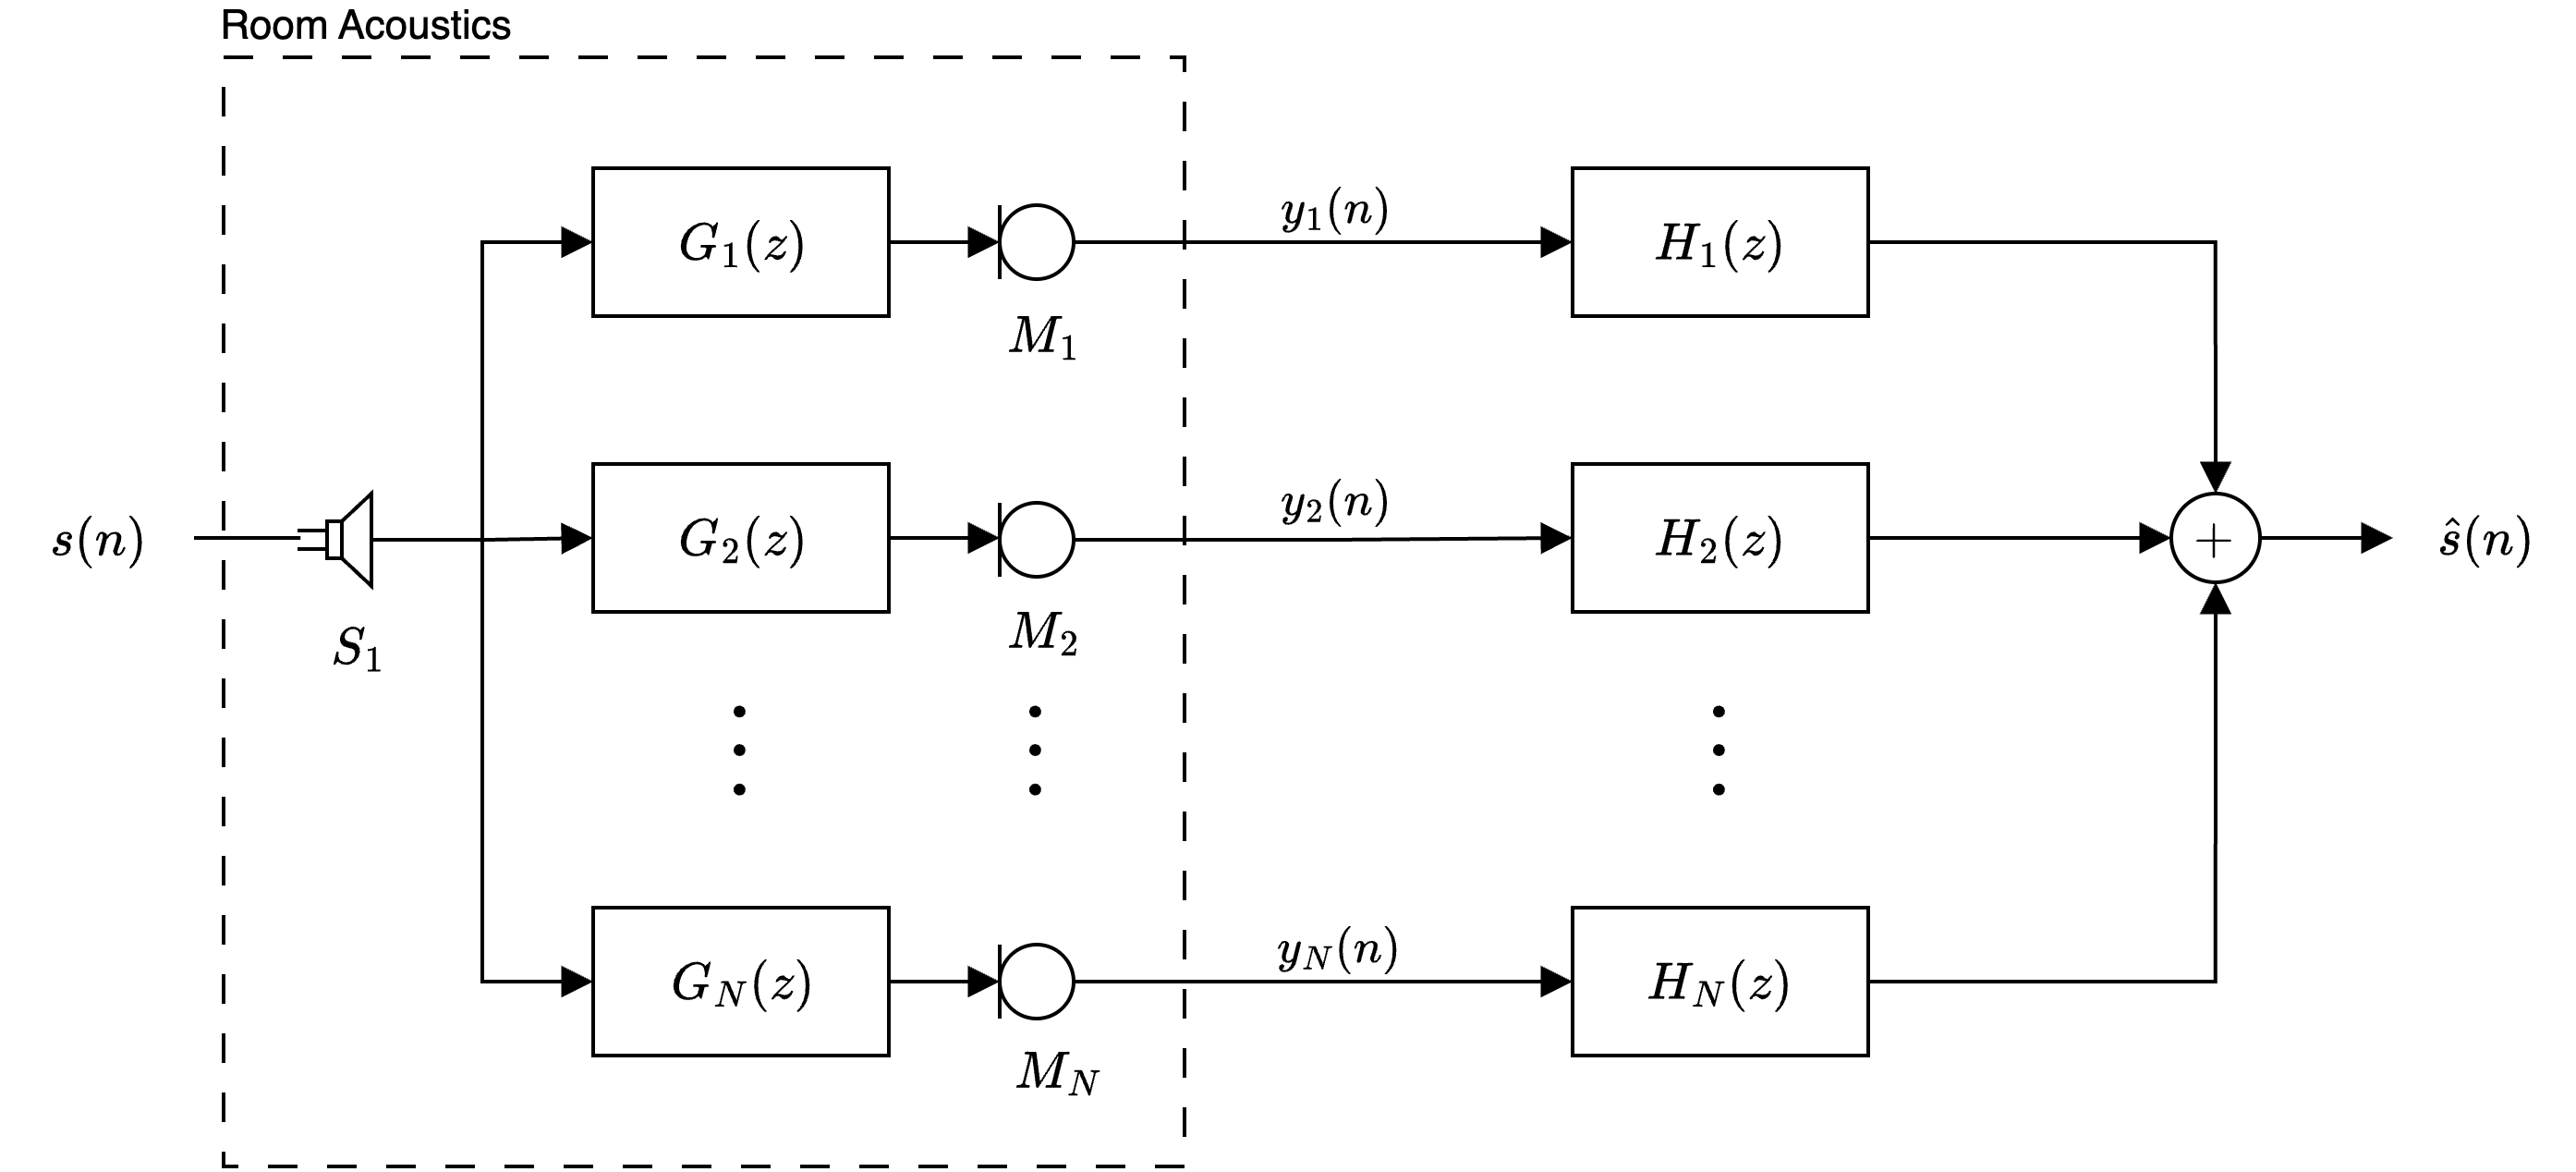
\includegraphics[width=\textwidth]{MINT_SIMO_Dereverb}
	\end{subfigure}
	\hfill
	\begin{subfigure}[b]{0.49\textwidth}
		\centering
		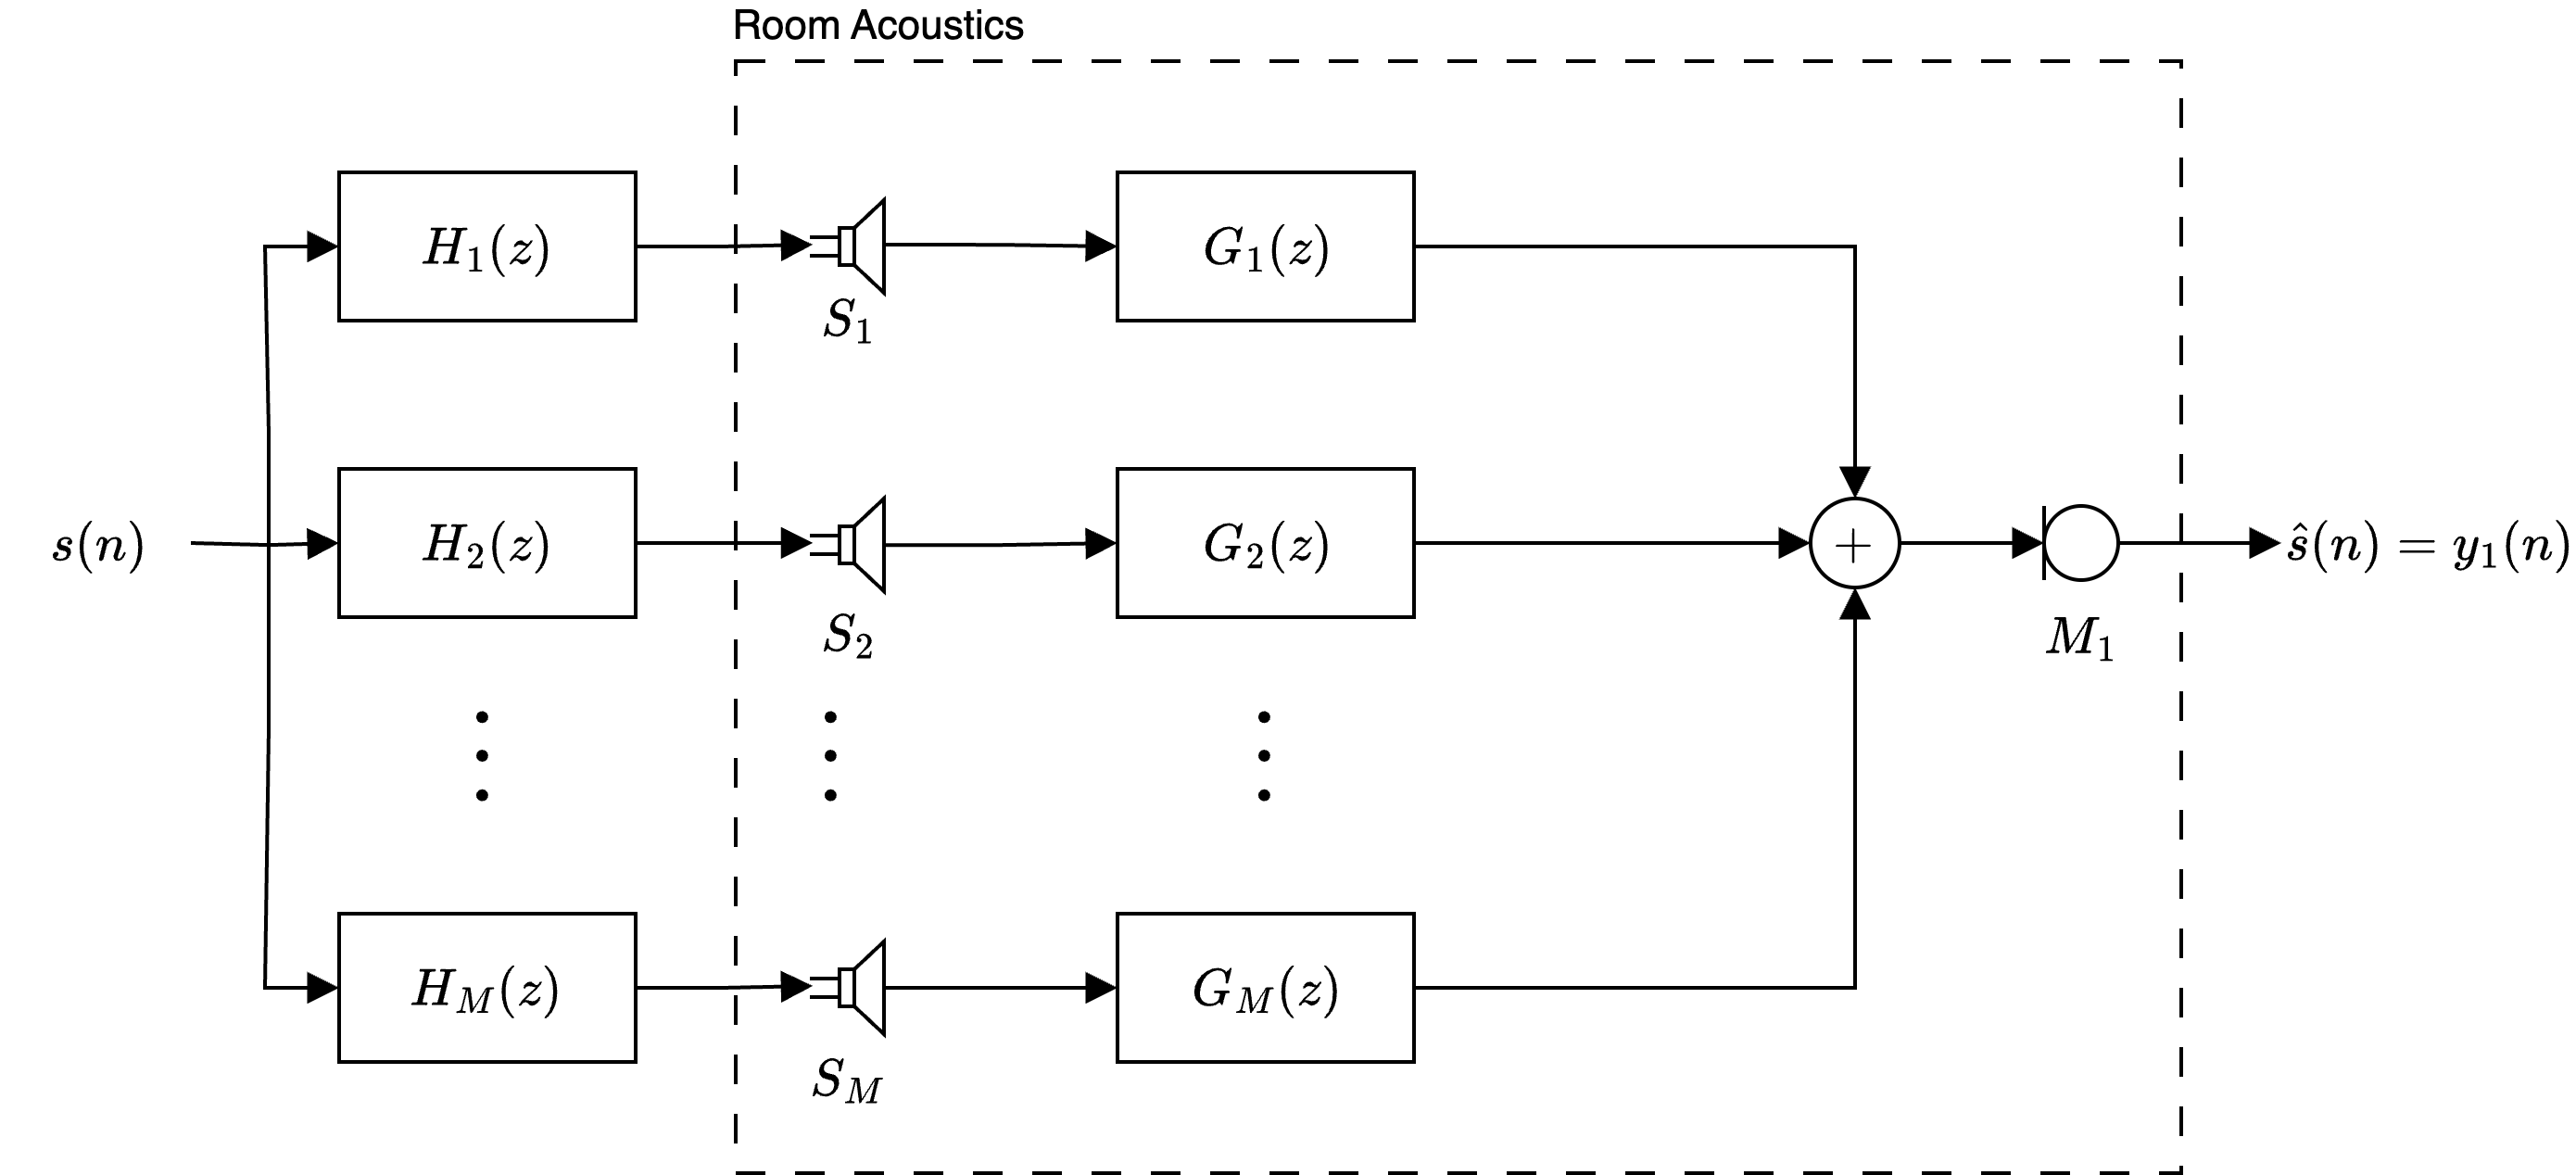
\includegraphics[width=\textwidth]{MINT_MISO_SoundReprod}
	\end{subfigure}
	\caption{Block diagram the formulations of MINT filtering: dereverberation (left) and sound reproduction (right)}
	\label{fig:MINT_Structures}
\end{figure}

Sound reproduction describes a multiple-input single-output (MISO) system, where each loudspeaker signal is pre-processed with a unique FIR equalizer so as to equalize the RTF at a certain location in the room. Dereverberation describes a single-input multiple-output (SIMO) system where the microphone signals are filtered and summed, with the intention obtaining a clean signal that can be played back elsewhere (e.g., a hearing aid loudspeaker inside the ear canal).

In the SIMO dereverberation case, which is relevant to this thesis, the solution can be derived as follows. Let $g_i(n)$ be the length-$n$ FIR RIR corresponding to acoustic RTF between the source loudspeaker and microphone $i$. Let $h_i(n)$ be the length-$m$ FIR equalizer applied to microphone $i$ before summation with the other channels. 

\begin{eqnarray}
	G_i(z) = Z\{g_i(n)\} = \sum_{k=0}^{n-1}g_i(k)z^{-k} \\
	H_i(z) = Z\{h_i(n)\} = \sum_{k=0}^{m-1}h_i(k)z^{-k} \\
\end{eqnarray}

The inverse filtering problem can be stated in matrix form as

\begin{eqnarray}
	\boldsymbol{G} \boldsymbol{h}=\boldsymbol{d} \label{eq:MINT_problem} \\
	%
	\boldsymbol{G} \boldsymbol{h} =
	\begin{bmatrix}
		\boldsymbol{G}_1 & \boldsymbol{G}_2 & \dots& \boldsymbol{G}_N
	\end{bmatrix} 
	\begin{bmatrix}
		\boldsymbol{h}_1 \\
		\boldsymbol{h}_2 \\
		\vdots \\
		\boldsymbol{h}_N \\
	\end{bmatrix}
	=
	\begin{bmatrix}
		d(0) \\
		d(1) \\
		\vdots \\
		d(m+n-2) \\
	\end{bmatrix} 
	=
	\boldsymbol{d}
\end{eqnarray}

\noindent
Where $\boldsymbol{h_i}$ is the vector form of the FIR equalizer applied to microphone $i$, i.e.,

\begin{eqnarray}
	\boldsymbol{h}_i = 
		\begin{bmatrix}
			h_i(0) & h_i(1) & \dots & h_i(m-1)
		\end{bmatrix}^T
\end{eqnarray}

\noindent
and $\boldsymbol{G}_i$ is the filter matrix (i.e., the Sylvester matrix) corresponding to the convolution of $g_i(n)$ with $h_i(n)$, i.e.,

\begin{eqnarray}
	\boldsymbol{G}_i = 
	\begin{bmatrix} 
		g_i(0)     & 0           & 0              & \dots    & 0  \\
		g_i(1)     & g_i(0)    & 0              & \dots    & 0  \\
		g_i(2)    & g_i(1)     & g_i(0)      & \dots    & 0  \\
		\vdots    & \vdots    & \vdots     & \ddots & \vdots  \\
		g_i(n-1) & g_i(n-2) & g_i(n-3) & \dots   & 0 \\
		0            & g_i(n-1)  & g_i(n-2) & \dots   & 0 \\
		0            & 0             & g_i(n-1
		111) & \dots   & 0 \\
		\vdots    & \vdots    & \vdots     & \ddots & \vdots  \\
		0            & 0             & 0             & \dots   & g_i(n-1) \\
	\end{bmatrix} 
	\in \mathbb{R}^{(m+n-1)\times m}
\end{eqnarray}

\noindent
To acheive perfect zero-delay equalization, the desired EIR should be $d(n)=\delta(n)$, and therefore

\begin{equation}
	\boldsymbol{d} =
		\begin{bmatrix}
			1 & 0 & \dots & 0
		\end{bmatrix}^T
\end{equation}

Since $\boldsymbol{G} \in \mathbb{R}^{(m+n-1)\times Nm}$, equation \ref{eq:MINT_problem} represents a problem with $m+n-1$ equations and $Nm$ variables. A perfect solution exists provided $\boldsymbol{G}$ is invertible, which requires that it is square and full rank. For $\boldsymbol{G}$ to be square, that the equalizer filter length, $m$, must be

\begin{equation}
	m = \frac{n-1}{N-1}
\end{equation}

\noindent
Provided $\boldsymbol{G}$ is full rank, the MINT can be computed as

\begin{equation}
	\boldsymbol{h} = \boldsymbol{G}^{-1}\boldsymbol{d}
\end{equation}

For $m < \frac{n-1}{N-1}$, the problem is overdetermined and no perfect solution exists, i.e., it can only be solved by least squares. However, for $m > \frac{n-1}{N-1}$, the problem is underdetermined and therefore has infinite perfect solutions provided its rank is greater than or equal to the number of columns/unknowns. In this case the pseudo-inverse can be used to select the minimum norm solution. I.e.,

\begin{equation}
	\boldsymbol{h} = \boldsymbol{G}^+\boldsymbol{d} = \boldsymbol{G}^T(\boldsymbol{G}\boldsymbol{G}^T)^{-1}\boldsymbol{d}
\end{equation}

\textbf{Confirm that this form of the psuedo inverse is required for solving an underdetermined system, and is different from the other form which is used for solving an overdetermined system (i.e., least squares)}

 Therefore, for the SIMO dereverberation case, the equalizer filter length, $m$ is required to be

\begin{equation}
	m >= \frac{n-1}{N-1}
\end{equation}

\noindent
where $m$ is the length of the individual FIR equalizers, $n$ is the length of the individual FIR channels, and $N$ is the number of microphones. Note that although the individual FIR channels are not necessarily the same length, they can be zero padded to the longest length.

Equivalently, for the MISO sound reproduction case, the equalizer filter length requirement was shown to be

\begin{equation}
	m >= \frac{n-1}{M-1}
\end{equation}

\noindent
where $M$ is the number of loudspeakers.


 \cite{miyoshi1986inverse} proved that in order to be invertible (i.e., in order for $\boldsymbol{G}$ to be full rank), there could not be any zeros that were common to all RTFs. It was therefore shown that a MINT equalizer can achieve perfect zero-delay equalization, even when the individual RTFs are non-minimum phase, provided the equalizer filter lengths are sufficiently long and the individual RTFs do not have common zeros anywhere in the z-plane. This result is different from single channel methods which only approach perfect equalization of non-minimum phase channels as the modeling delay approaches infinity. 
 
 It is interesting to note that FIR channels would inheritly have inverse filters that are all-pole and therefore IIR. Single channel FIR equalization of a FIR channel will thus always be approximate, even if the channel is minimum phase. This makes sense intuitively, but \cite{miyoshi1986inverse} also proved this numerically by demonstrating that the matrix formulation of the single channel equalization problem is always overdetermined regardless of equalizer filter length. Remarkably, the MINT can acheive perfect equalization of a FIR channel with individual FIR equalizer filters that are shorter in length than the FIR channels. It is important to remember that real RTFs are not generally speaking FIR, so the MINT is still approximate. However, for a sufficiently long FIR measurement of the true RIR, the residual reflections may be considered negligible.The MINT was proven to greatly outperform the single channel least squares equalization method, acheiving more than \qty{40}{\decibel} additional reverberation attenuation accross all frequencies.
 
In an extended discussion of the MINT,  \cite{miyoshi1988inverse} explored the MIMO case for sound reproduction. They proved that it is possible to perform sound reproduction at $N$ listening positions using $M$ loudspeakers provided the channels had no common zeros,

\begin{equation}
	M > N
\end{equation}

and

\begin{equation}
	m >= \frac{N(n-1)}{M-N}
\end{equation}

In an extension of the MINT, \cite{nakajima1997sound} proposed the indefinite MINT filter (IMF) which exploits the additional degrees of freedom gained when the FIR equalizer length $m$ is strictly greater than its minimum required length. In this underdetermined case, there are infinite solutions. While the classical MINT recommended using the pseudo inverse to compute the minimum norm solution, IMF makes use of the additional degrees to equalize nearby points. This has the effect of expanding the equalized zone and improving robustness to spatial variation of the RTF.

\subsubsection{Perceptually Motivated Room Response Equalization}

Several authors have proposed extensions to RTF equalization appraoches which constrain the solution to improve perception rather than simply to equalize the channel. This includes the partial MINT \citep[i.e., PMINT][]{kodrasi2012robust}, the relaxed multichannel least-squares \citep{zhang2010use}, and channel shortening \citep{kallinger2006multi}.


\subsection{Blind Deconvolution Problem}

The RTF equalization approaches discussed in the previous section were reliant on having prior knowledge of the RIR (e.g., by measurement). However, typically in the context of dereverberation, the RIR is not known and must be estimated by other means. The approaches to estimation of a unknown linear system can be divided into supervised methods (i.e., trained/supervised deconvolution) and unsupervised methods (i.e., blind/unsupervised deconvolution).

\subsubsection{The Wiener Filter (Supervised Optimal Filtering)} \label{wiener_filter}

Traditional supervised optimal filtering is formulated as the selection of a filter $H(z)$ which, for a known input sequence $x(n)$, produces a output $y(n)$ that is optimally close (in a mean-squared error sense) to a desired/reference signal $d(n)$. I.e., the goal is to design $H(z)$ such that the energy in the error signal $e(n) = d(n)-y(n)$ is minimized. 

\begin{figure}[H]
	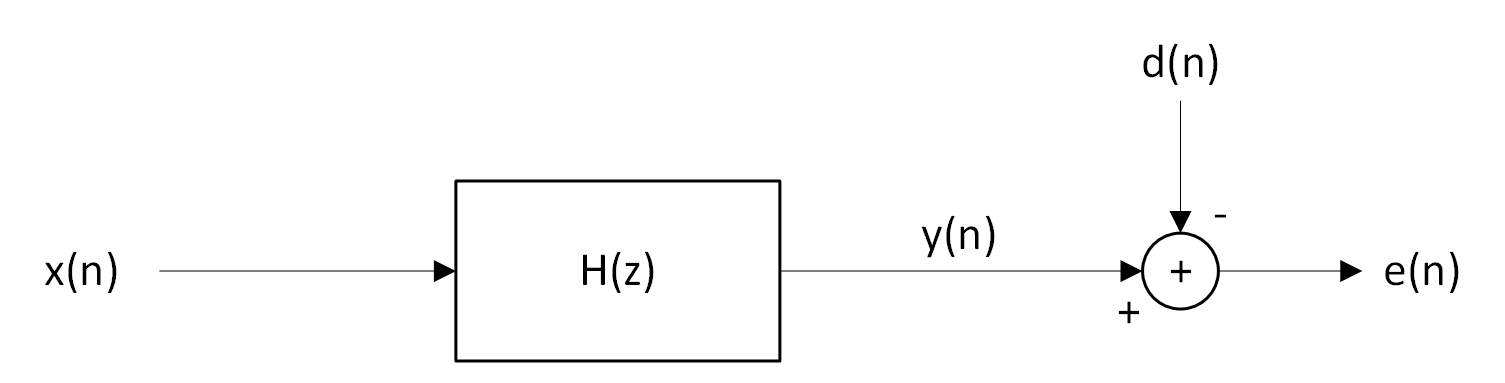
\includegraphics[width = 0.6\textwidth]{WienerFilter}
	\centering
	\caption{Block diagram for supervised optimal filtering, which attempts to produce a desired output, $d(n)$, from a known input, $x(n)$}
	\label{fig:WienerFilterProblem}
\end{figure}

The derivation for this optimal solution, originally proposed by \cite{wiener1949extrapolation}, is performed in a stochastic framework using expectations for computing mean-squared error. The resulting solution is referred to as the Wiener filter. Considering a length-$N$ FIR filter, $H(z)=\sum_{k=0}^{N-1}h_k z^{-k}$, this is mathematically formulated as

\begin{eqnarray}
	\boldsymbol{x}(n) = 
	\begin{bmatrix}
		x(n) & x(n-1) & \dots & x(n-N+1)
	\end{bmatrix}^T \\
	%
	\boldsymbol{h} = 
	\begin{bmatrix}
		h_0^* & h_1^* & \dots & h_{N-1}^*
	\end{bmatrix}^T \\
	%
	e(n)=d(n) - y(n) = d(n) - \boldsymbol{h}^H\boldsymbol{x}(n) \\
	%
	J(\boldsymbol{h}) = E\left[ \left| e(n) \right|^2 \right] = E\left[e(n)e^H(n)\right] \\
	%
	J(\boldsymbol{h}) = E\left[
	\left(d(n) - \boldsymbol{h}^H\boldsymbol{x}(n)\right)
	\left(d(n) - \boldsymbol{h}^H\boldsymbol{x}(n)\right)^H
	\right] \label{eq:wiener_cost_fn_0} \\
	% 
	J(\boldsymbol{h}) = \sigma_d^2 - \boldsymbol{h}^H\boldsymbol{p} - \boldsymbol{h}^T\boldsymbol{p}^*+\boldsymbol{h}^H R \boldsymbol{h} \label{eq:wiener_quadratic}
\end{eqnarray}

\noindent
Where $\boldsymbol{p} = E \left[ \boldsymbol{x}(n)d^*(n) \right]$ is the cross-correlation vector between the input process and the desired/reference process, and $\boldsymbol{R} = E \left[ \boldsymbol{x}(n)\boldsymbol{x}^H (n) \right]$ is the autocorrelation matrix of the input process.

Since the highest-order factor in Equation \ref{eq:wiener_quadratic}, i.e., $\boldsymbol{h}^H \boldsymbol{R} \boldsymbol{h}$ is a quadratic form and the autocorrelation matrix $\boldsymbol{R}$ is Hermitian positive semidefinite (assuming the input process is stationary), $J(\boldsymbol{h})$ represents a quadratic bowl in $N+1$ dimensions with exactly one global minimum. This minimum can be found by taking the derivative of the cost function and setting it equal to zero. I.e.,


\begin{eqnarray}
	%
	\frac{\partial J(\boldsymbol{h})}{\partial \boldsymbol{h}^*}=0 \\
	%
	\boldsymbol{R} \boldsymbol{h} = \boldsymbol{p} \label{eq:wiener_hopf}
\end{eqnarray}

Equation \ref{eq:wiener_hopf} is referred to as the Wiener-Hopf equation and can be solved by any number of methods for solving systems of linear equations. This equation can also be viewed as a stochastic extension of the LS normal equations, and equivalently the Yule-Walker equations in linear prediction. I.e., the Wiener filter is optimal for known stationary processes, whereas the LS normal equations produce a filter that is optimal for a known set of data. 

In practice the statistical correlation functions that make up $\boldsymbol{p}$ and $\boldsymbol{R}$ in the Wiener-Hopf equations must be estimated from a finite set of data, and given certain short-term estimation techniques, the Wiener-Hopf equations become identical to the LS normal equations.

The conditioning of the Wiener-Hopf equation is dictated by the eigenvalue spread of the autocorrelation matrix, $\boldsymbol{R}$, which has been shown to be correlated to the dynamic range of the input spectrum (i.e., the “peakiness”). When the input process is white, the eigenvalue spread is equal to 1, and the autocorrelation matrix is the identity matrix. When the input sequence is coloured, the non-zero off-diagonal autocorrelation values result in a larger eigenvalue spread (i.e., higher condition number), which can lead to a less numerically stable solution.

In practice there is always additional sensor noise present which interferes with the measured input, $x(n)$, and/or error signal, $e(n)$. This interference leads to additional misadjustments of the final solution due to distortions in the autocorrelation matrix.

The Wiener filter has also been extended to the optimal derivation of an IIR filter (i.e., the unconstrained Wiener filter), which results in the following frequency domain solution.

\begin{equation}
	\boldsymbol{h}(e^{j\omega}) = \frac{\Phi_{dx}(e^{j\omega})}{\Phi_{xx}(e^{j\omega})}
\end{equation}

\noindent
Where $\Phi_{dx}(e^{j\omega})$ is the cross-PSD of $d(n)$ and $x(n)$, and $\Phi_{xx}(e^{j\omega})$ is the PSD of $x(n)$.

The Wiener filter and all resulting adaptive extensions can be applied to both transversal filters (as described above) and linear combiners (e.g., beamforming). 

\subsubsection{Supervised Adaptive Filtering}

To allow tracking of time-varying systems, adaptive algorithms have been proposed which aim to converge on the Wiener filter. Adaptive filtering theory leverages the fact that the MSE cost function forms a quadratic error surface, and generally performs some form of gradient descent to make iterative steps towards the optimal solution. A detailed discussion of the details of adaptive filtering theory can be found in \cite{farhang2013adaptive}, but an overview of the most common algorithms will be provided below.

The steepest descent algorithm (SD) estimates the gradient,

\begin{equation}
	\bold{\nabla} J(\boldsymbol{h}) = 
	\frac{\partial J(\boldsymbol{h})}{\partial \boldsymbol{h}^*} = \frac{\partial E\left[e(n)e^H(n)\right]}{\partial \boldsymbol{h}^*} \\
\end{equation}


\noindent
of the MSE error surface and steps in the direction opposite to it. The shape of the error surface is dictated by the eigenvalue spread of the autocorrelation matrix for the input sequence, and therefore also the peakiness of the input spectrum. For a white input spectrum, the equal-MSE contours for the error surface are circular, and the negative gradient points directly towards the optimal solution. For more coloured/peaky spectra, the equal-MSE contours of the error surface become elongated, resulting in a negative gradient which does not point directly towards the optimal solution. The Newton descent (ND) algorithm modified SD by deriving the optimal vector-valued step such that the direction of iteration always points directly to the optimal solution regardless of eigenvalue spread

Both SD and ND require estimation of the autocorrelation matrix, $\boldsymbol{R}$, and the cross-correlation vector, $\boldsymbol{p}$. This is computationally expensive, and also it is common for the desired/reference process to be unknown (i.e., only the error sequence is known), making the cross-correlation vector, $\boldsymbol{p}$, impossible to estimate. This motivated the usage of the stochastic gradient which is computed solely based on the measured error sequence. The stochastic gradient, defined as

\begin{equation}
	\frac{\partial \left(e(n)e^H(n)\right)}{\partial \boldsymbol{h}^*} = - \boldsymbol{x}(n)e^*(n) \\
\end{equation},

\noindent
represents an instaneous stochastic estimate of the true gradient, $ \frac{\partial E\left[e(n)e^H(n)\right]}{\partial \boldsymbol{h}^*} $.

The commonly used least-mean-squares (LMS) algorithm, steps in the direction of the negative stochastic gradient, using the filter update equation

\begin{equation}
	\boldsymbol{h}(n+1) =
	 \boldsymbol{h}(n) - \mu 	\frac{\partial \left(e(n)e^H(n)\right)}{\partial \boldsymbol{h}^*(n)} =
	 \boldsymbol{h}(n) + \mu \boldsymbol{x}(n)e^*(n)
\end{equation}

\noindent
Where $\mu$ is the step size used to control the rate of adaptation. 

The LMS algorithm is very low complexity, does not require prior knowledge/estimation of the statistics of the input process or desired/reference process, and its adaptation trajectory has been shown to match (in the ensemble average) that of the steepest descent algorithm. However, the step size must be carefully selected based an estimate of the eigenvalue spread of the input process to ensure stable convergence.

The Normalized LMS (NLMS) algorithm added a step size that was normalized based on input signal energy so that a standard step size of $\mu=1$ could always be considered optimal (in practice $\mu < 1$ is often required due to numerical error). The NLMS update equation is

\begin{equation}
	\boldsymbol{h}(n+1) =
	\boldsymbol{h}(n) + \mu (n)\boldsymbol{x}(n)e^*(n) = 
	\boldsymbol{h}(n) + \frac{\mu}{\boldsymbol{x}^H(n)\boldsymbol{x}(n) + \varphi} \boldsymbol{x}(n)e^*(n)
\end{equation}

\noindent
Where $\varphi$ is a small regularization offset used to avoid filter divergence during periods of very low input energy (i.e., to avoid effective division by zero).

Separate from gradient-based algorithms described above, the recursive least squares (RLS) algorithm forms an adaptive extension of least squares optimization. This data-centric approach minimizes deterministic total-squared-error for the specific data observed. RLS performs LS optimization over all data observed since the start of time, with an added forgetting factor to allow tracking of time-varying systems.

As was the case with Wiener filtering, in practice there is additional sensor noise present in the measured input signal, $x(n)$, and/or error signal, $e(n)$, which interferes with the adaptation and leads to misadjustments. This can be particularly problematic when the interfering noise is correlated with itself.

All adaptive algorithms are derived in the complex domain to allow implementation in the frequency domain and subband domain. Adaptation in the frequency/subband domain is often desirable for computational efficiency and to allow control of the adaptation on a frequency-selective basis. Additionally, convergence tends to be faster in the frequency/subband since narrowband signals tend to have flatter spectra than wideband signals. However, the DFT/Inverse DFT or subband filterbank adds computational complexity and memory of its own, and increases system latency which may not be desirable.


\subsubsection{Blind Deconvolution Challenges}

When applied to system equalization (e.g., RTF equalization), as depicted in Figure \ref{fig:supervised_inverse_filter}, the desired/reference signal is the input to the unknown system, i.e., $d(n)=s(n)$, and input to the equalizer filter, $H(z)$, is the output of the unknown system, i.e., $x(n)=s(n)*h(n)$. 

\begin{figure}[H]
	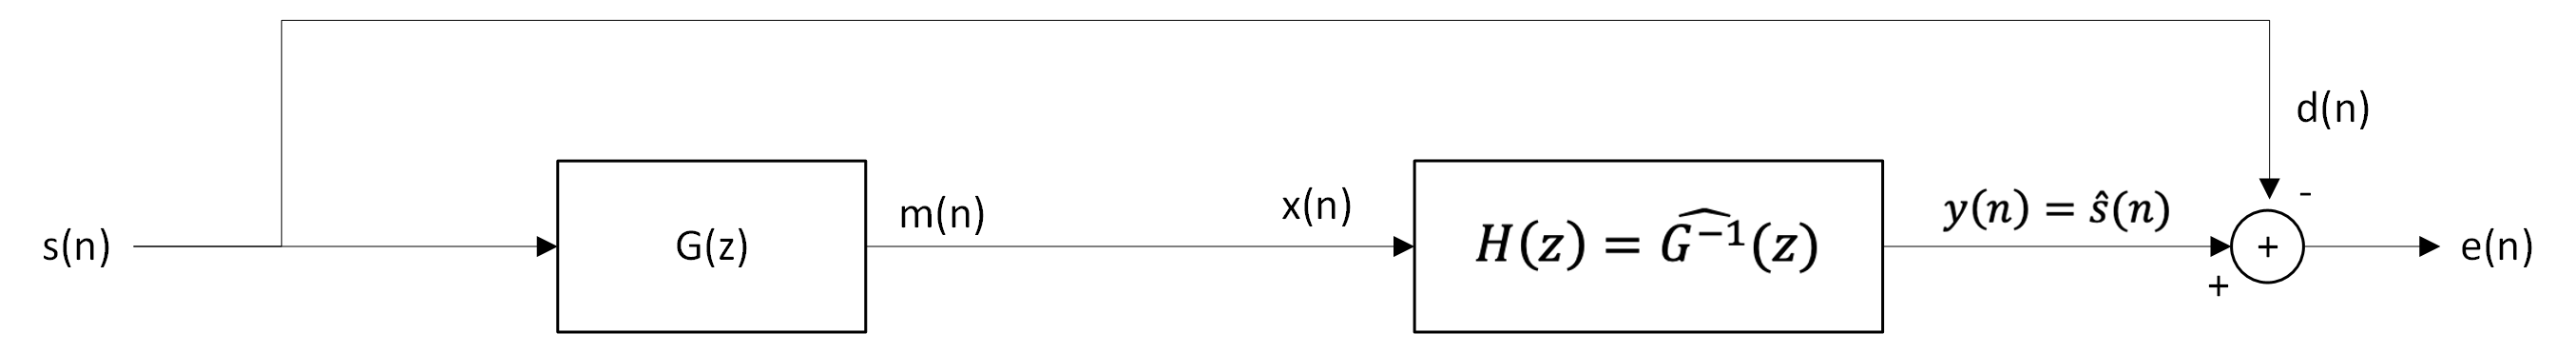
\includegraphics[width = \textwidth]{supervised_inverse_filter}
	\centering
	\caption{Block diagram for supervised inverse filtering / equalization, which attempts to produce reproduce the known input, $s(n)$, to an unknown system $G(z)$, from the measured system output, $y(n)$, using a filter, $H(z)$}
	\label{fig:supervised_inverse_filter}
\end{figure}

Blind deconvolution (i.e., unsupervised inverse filtering) refers to the problem of inverse filtering when the input, $s(n)$, to the unknown system, $G(z)$, is unknown as well. This generally requires two stages: unsupervized estimation of the unknown  (i.e., blind system identification, or BSI), and inverse filtering. In terms fo the previous discussion, this implies that the desired output the equalizer being designed ($d(n)$ in Figure \ref{fig:WienerFilterProblem}) is unknown, and equivalently the error signal ($e(n)$) is also unknown. For completeness, measurement noise, $v(n)$, is included.

\begin{figure}[H]
	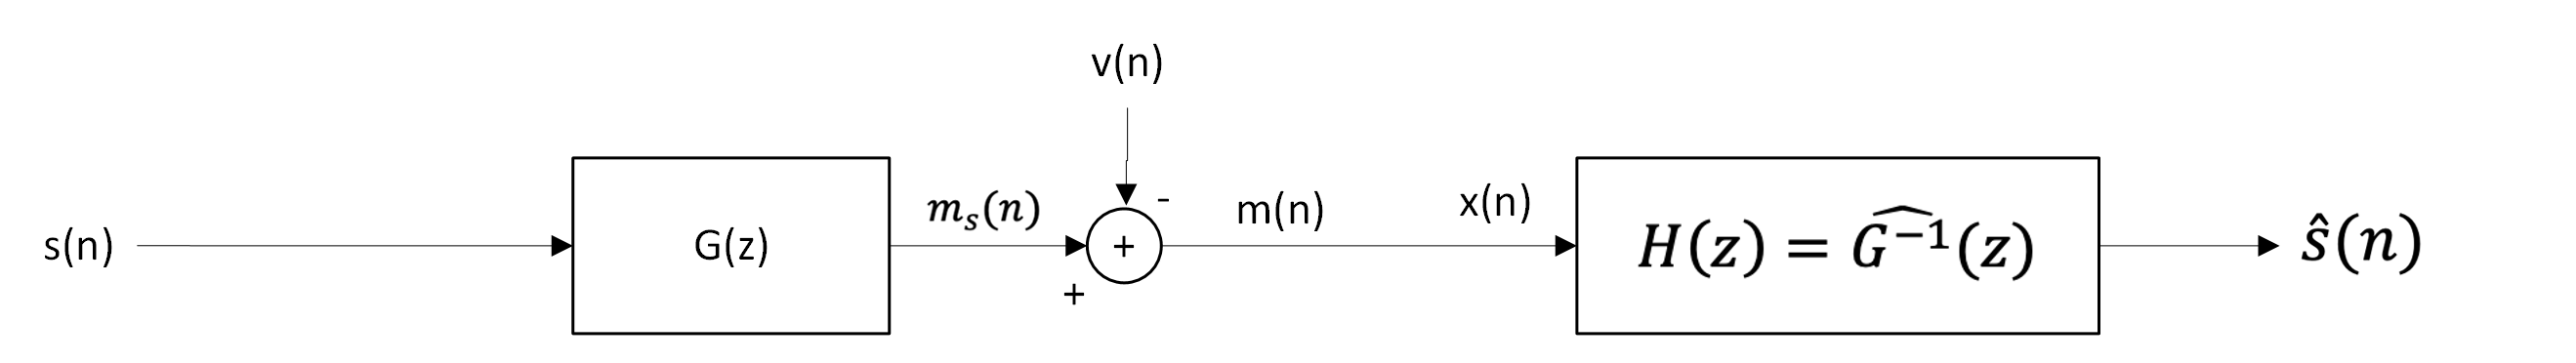
\includegraphics[width = \textwidth]{blind_deconvolution}
	\centering
	\caption{Block diagram for supervised blind deconvolution, which attempts to produce reproduce the unknown input, $s(n)$, to an unknown system $G(z)$, from the measured system output, $y(n)$, including additive noise $v(n)$, using a filter, $H(z)$}
	\label{fig:blind_deconvolution}
\end{figure}

Speech dereverberation is generally a blind problem since the source is a human talker, and the corresponding speech signal is only measured at the listening point (i.e., only the RTF system output is available). This creates a challenging problem since the system input, $s(n)$, and system itself, $G(z)$, are both unknown and must be derived from the measured signal at the output, $y(n)$ (i.e., microphone signal). Therefore, there is an ambiguity as to whether the poles and zeros of the measured output signal correspond to the input signal or the system.

In the context of blind wireless channel equalization, the unknown source often falls into a discrete set of known symbols that are stationary within a symbol period. This can be exploited to make assumptions about the source when estimating the system. Conversely, in speech dereverberation, the speech signal is virtually arbitrary and highly non-stationary, making the problem even more challenging.

Additionally, as discussed in Section \ref{RIR_Invertibility}, reverberant channels vary significantly with respect to spatial location and slight misadjustments to the equalizer can result in making the effects of reverberation worse. This spatial variance results in a highly time-varying channel, which must be tracked adaptively. Also, as discussed, RTFs tend to be non-minimum-phase thus not having a causal stable single-channel inverse, and may have strong or perfect zeros which can result in severe narrowband noise amplification.

As with traditional supervised system equalization, interfering noise can result in miconvergence of the inverse filter, and must be handled accordingly.

Lastly, since reverberation times can be in the order of several seconds, resulting in sampled RIRs spanning thousands or even tens of thousands of taps, computations in reverberation cancellation also tend to be very complex and sensitive to numerical error.

\subsubsection{Practical Blind Deconvolution in Wireless Systems}

The topic of blind deconvolution originated in geophysics and wireless communication, and has been studied extensively in these fields. A full discussion of the topic of blind wireless channel inversion can be found in \cite{ding2018blind}, but some of the most common practical approaches will be summarized here. As will be shown, these approaches generally rely on assumptions about the source signal which do not hold in the context of speech dereverberation.

In wireless systems, where the input signal is controlled by a radio base station and the output is detected by a mobile phone, often a periodic training sequence (i.e., a reference symbol) is used as a reference for performing periodic supervised adaptive channel estimation. However to provide continuous tracking of the time-varying channel without using too much channel bandwidth for reference symbols, additional unsupervised adaption is often employed.

The first unsupervised approach, proposed by \cite{lucky1965automatic}, was the so-called decision-directed approach, in which the system which toggled between supervised and unsupervised adaptation periodically. A non-linear decision device at the output of the equalizer was used to select the most likely symbol (e.g., closest symbol in the magnitude-phase symbol constellation), and during periods of unsupervised adaptation this estimated symbol was used as the desired equalizer output to make adaptations. This concept was highly reliant on the theory of Bussgang statistics which allows important assumptions about the statistics of a stochastic process before and after a memoryless non-linear operation. This approach has been shown to work well provided the channel is slowly time-varying and there is minimal misconvergence during supervised training so that deviations during unsupervised training are minimal. Building on this concept the Sato method \citep{sato1975method} and the Constant Modulus algorithm \citep{godard1980self} were proposed which improved robustness to larger deviations by adapting using an error metric between measured signal and the set of possible symbols, instead of a hard symbol decision. 

These algorithms laid the groundwork for the approaches used in practice, most of which rely on the fact that the transmitted symbols may only fall into a set of known symbols. This assumption of course does not hold for speech dereverberation where the source signal is highly non-stationary speech. Truly blind adaptation without exploiting knowledge of a symbol dictionary, which has applications in speech dereverberation, will be explored in the subsequent sections.

\subsubsection{SOS and HOS Methods for Blind System Identification}

Techniques for BSI can generally by categorized by their usage of second order statistics (SOS) or higher order statistics (HOS). 

It is well understood that SOS such as autocorrelation and power spectrum only capture the magnitude information of a signal, and do not directly capture any phase information. Referring back to Figure \ref{fig:blind_deconvolution}, the power spectrum of the system output, $y(n)$, (neglecting noise) is given by

\begin{equation}
	S_{yy}(\omega) = |G(\omega)|^2 S_{ss}(\omega)
\end{equation}

\noindent
Therefore, if only the SOS of the system output is known, then only the magnitude response of the channel, $|G(\omega)|$, can be identified. For this reason, SOS methods for BSI are limited in their ability to perfectly identify the true underlying system. Since the phase response of an RTF contains significant reverberant energy (Section \ref{homomorphic_eq}), this has a strong impact on dereverberation performance. Also note that correct identification of $|G(\omega)|$ from only the SOS of the system's output ($S_{yy}(\omega)$) additionally requires knowledge of the SOS of the system's input ($S_{ss}(\omega)$). As such, truly blind estimation of $|G(\omega)|$ requires that the input is white and stationary (i.e., independent and identically distributed, i.i.d. up to the 2nd order).

In the seminal work by \cite{giannakis1989identification}, it was shown that the complete magnitude and phase information of an LTI system are captured in the HOS of the system's output. Specifically, it was shown that the magnitude and phase information are retreivable from the $k$-order cumulant or the $(k-1)$-order polyspectrum of the system's output for $k>2$, provided the input is non-Gaussian (i.e., it has non-zero HOS). Similar to the SOS case, identification of the system, $G(z)$, from only the HOS of the system's output requires knowledge of the HOS of the input, or equivalently assumes that the input is i.i.d. up to the kth order. If the input is not i.i.d., the identified system will include the source statistics, and therefore the designed equalizer will whiten the source as well. To avoid this undesired result, additional processing is needed to estimate and restore the source spectrum.

In practice, HOS methods are not often used for dereverberation due to the massive amount of signal data needed to reduce the high level of variance that arises in numerical estimates of HOS. This data constraint results in high computational complexity, and greatly reduces the ability of algorithms to track time-varying channels.
	
\subsubsection{Multichannel SOS Methods for Blind System Identification} \label{mc_sos_bsi}

In the previous section, it was explained that SOS do not capture phase information, which can severely impact dereverberation performance. However, it has been shown that using multiple channels, partial phase information can be captured. Originally demonstrated by \cite{slock1994blind}, the spatial diversity gained from a multichannel setup gives rise to spatial cross-correlations from which relative phase information can be extracted. In the context of dereverberation, this is realized using multiple microphones. Since only the relative phase is known, the system can only be identified up to a linear-phase term.

Additionally, the spatial diversity gained by using multiple microphones provides a mechanism for mitigating the source/filter ambiguity that is inherit to the BSI problem. Intuitively, if the poles and zeros each microphone signals are known (or can be estimated), the source components will be common to all microphone signals, while the channel/filter components will be different for each microphone. Therefore, it is possible to uniquely identify the channel RTFs provided there are no poles or zeros that are common to all channels.

As discussed in Section \ref{MINT}, the usage of multiple channels in equalizer design also makes it possible to perfectly equalize non-minimum phase systems (i.e., a MINT equalizer). This is possible provided the MINT conditions are met, i.e., the individual channel RTFs do not share common zeros and the individual FIR equalizer filters are of length $m >= \frac{n-1}{N-1}$, where $n$ is the length of the individual RIRs and N is the number of microphones. Mutlichannel SOS methods for BSI can thus be viewed as a blind estimation of the MINT equalizer.

In summary, using multiple microphones, it is possible to identify an arbitrary multichannel RTF from only it's output signals for any arbitrary source signal, provided the individual channels do not share common poles/zeros. Using a multichannel inverse filter, it is also possible to perfectly equalize this channel up to a gain factor and linear-phase term provided the MINT conditions are met. These properties, and the relatively small amount of data required to compute SOS, have given rise to a number of blind deconvolution methods for derverberation, which will be discussed in the following section.

\subsection{Multichannel SOS Methods for Reverberation Cancellation}

This section outlines existing methods for dereverberation by blind deconvolution using multichannel SOS methods for BSI. While all the following methods rely on multichannel SOS to separate the poles and zeros of the RTF from those of the source signal, they differ in the details of how this is done.

The Multichannel equalization problem is shown in Figure \ref{fig:MC_EQ}

\begin{figure}[H]
	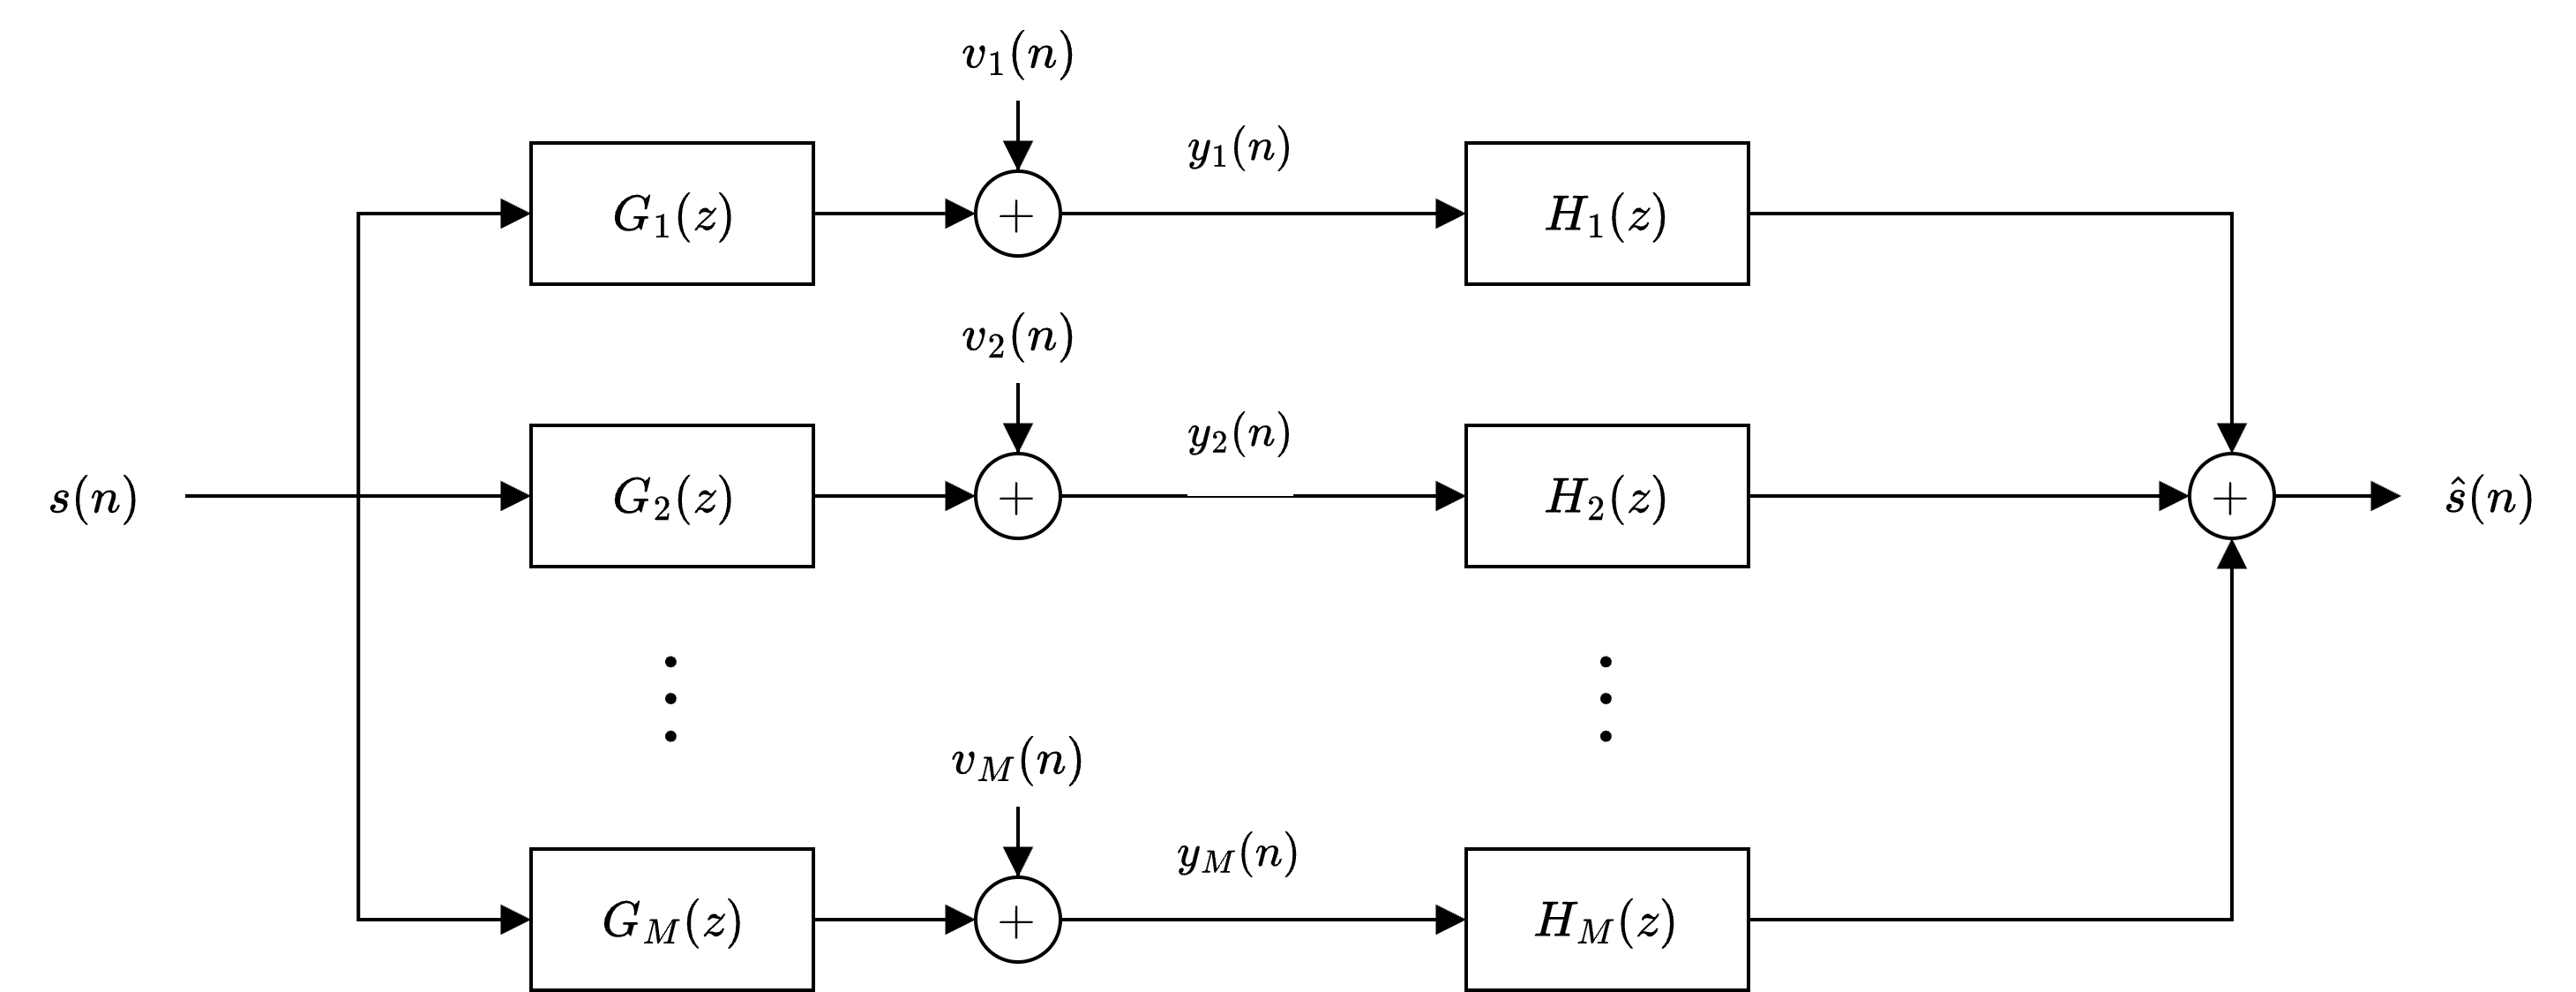
\includegraphics[width = \textwidth]{MC_EQ}
	\centering
	\caption{Block diagram for multichannel inverse filtering, which attempts to produce reproduce the known input, $s(n)$, to an unknown multichannel system $\{G_1(z), G_2(z), \dots, G_M(z)\}$, by filtering and summing the $M$ microphone signals, $\{y_1(n), y_2(n), \dots, y_M(n)\}$, with a set of FIR filters, $\{H_1(z), H_2(z), \dots, H_M(z)\}$}.
	\label{fig:MC_EQ}
\end{figure}

Like in Section \ref{MINT}, $G_k(z)$ will be used to denote the RTF from the source to the $k$th microphone, and $H_k(z)$ will be used to denote the FIR equalizer filter applied to microphone signal $k$ before summation with the other channels. Note that in this section $M$ will be used to denote the number of microphones/channels instead of $N$.


\subsubsection{Homomorphic Deconvolution}

One of the earliest proposed methods to blind deconvolution was accomplished in the complex cepstral domain \citep{oppenheim1976digital}. The complex cepstrum of a clean speech signal has been shown to be concentrated around the zero quefrencies, while complex cepstrum of the RIR tend to be concentrated at higher quefrencies. As such a simmple single-channel blind deconvolution technique consists of applying a window function (i.e., a short-pass lifter) to the complex cepstrum which attenuates the higher quefrencies. However, this effectively results in a minimum phase modeling of the system, which severely limits dereverberation performance. \cite{petropulu1994cepstrum} proposed a multichannel extension of this approach, and showed that an arbitrary mixed-phase RIR could be estimated from just the phases of two microphone signals. However, all homomorphic deconvolution methods tend to lead to severe speech distortions, and their performance is severely limited by the selection of the window function cutoff. 


\subsubsection{Subspace Methods}

Several methods have been proposed which build on a key observation from \cite{gurelli1995evam} that the RIRs of multiple channels can be extracted from the null space of the multichannel microphone data matrix. This was originally demonstrated in a two-channel noise-free configuration, where a source signal $s(n)$ is passed through two channels with RIRs $g_1(n)$ and $g_2(n)$, producing microphone signals,$y_1(n)$ and $y_2(n)$.

\noindent
\begin{eqnarray}
	y_1(n) = s(n)*g_1(n) \\
	y_2(n) = s(n)*g_2(n)
\end{eqnarray}

Conceptually, if each RIR is applied as a filter to the opposite microphone signal, the difference between the resulting signals should be zero. I.e., the so-called cross relation equality,

\noindent
\begin{equation}
	y_1(n)*g_2(n) - y_2(n)*g_1(n) = s(n)*g_1(n)*g_2(n) - s(n)*g_2(n)*g_1(n) = 0 \label{eq:cross_relation}
\end{equation}

\cite{gurelli1995evam} proved that the RIRs were consequently identical to the null space eigen-vectors of the multichannel data matrix (i.e., the data matrix of $y_1(n)$ and $y_2(n)$). A similar proof was shown to hold for an arbitrary number of channels. 

In the presence of noise, the multichannel data matrix generally does not have a null space since Equation \ref{eq:cross_relation} will not produce a difference of zero. Instead, the RIRs are extracted from the so-called "noise subspace" which is defined to have the smallest eigenvalues (i.e., minimizes cross-relation error).

Several more practical algorithms have been proposed to more heuristically minimize the cross-relation error, often using an adpative algorithm such as LMS, NLMS or RLS \citep[][]{identification1995least, huang2003class, huang2002adaptive}.

In addition to the requirements for BSI by use of SOS as specified in Section \ref{mc_sos_bsi}, this method also requires that the channel orders are known exactly so that the multichannel data matrix can be sized correctly. If the channel orders are over-estimated, the produced RIR estimates will include a common term of arbitrary extra zeros ($e(n)$), since

\begin{equation}
	s(n)*g_1(n)*g_2(n)*e(n) - s(n)*g_2(n)*g_1(n)*e(n) = 0
\end{equation}

\noindent
which will degrade performance. This is a severe limitation of technique, and for this reason subspace methods are not often useful in practice.


\subsubsection{Multichannel Linear Prediction Methods} \label{section_dap}

As discussed in Section \ref{linear_prediction}, linear prediction models speech as an autoregressive process, and consequently the prediction error filter ($A(z)=1-\sum_{k=1}^{p}a_k x^{-k}$) removes autocorrelation from the signals and thus acts as a whitening filter. Conceptually we can model a speech signal, $s(n)$, as the excitation of an all-pole filter with an uncorrelated input sequence, 

\begin{equation}
	S(z)=Z\{s(n)\}=U(z) \frac{1}{1 - \sum_{k=1}^{p}a_k z^{-k}}  = U(z) S_{\mathrm{AP}}(z)
\end{equation}

\noindent
where $S_{AP}(z)$ is an all-pole filter encapsulating all autocorrelation in $s(n)$, and $U(z)$ is the Z-transform of the uncorrelated residual part of $s(n)$  that does not fit the autoregressive model. The linear prediction "inverse filter" ($\frac{1}{A(z)} =\frac{1}{1 - \sum_{k=1}^{p}\alpha_k z^{-k}}$)  is an estimate of that all-pole model (i.e., of $S_{\mathrm{AP}}(z) = \frac{1}{1 - \sum_{k=1}^{p}a_k z^{-k}})$). 

If we extend this modeling concept to a reverberant speech signal, $y(n)$, that is produced by filtering $s(n)$ with an RIR, $g(n)$, we get

\begin{equation}
	Y(z) = S(z) G(z) = \tilde{U}(z) S_{\mathrm{AP}}(z) G_{\mathrm{AP}}(z)
\end{equation}


\noindent
where $G_{\mathrm{AP}}(z)$ is an all-pole model of $G(z)$, and $\tilde{U}(z)$ encapsulates the uncorrelated residual part of both $s(n)$  and $g(n)$ that does not fit the autoregressive model. As described in Section \ref{dt_speech_model}, an arbitrary transfer function can be perfectly represented by an infinite number of poles, and can be represented reasonably with a sufficient number of poles.

Since linear prediction estimates $S_{\mathrm{AP}}(z)G_{\mathrm{AP}}(z)$ without any knowledge of the input sequence $s(n)$, it effectively performs blind system identification, and the prediction error filter fascilitates blind deconvolution. However, the prediction error filter will also remove the autoregressive properties of the source signal, which will result in over-whitening of the speech signal. The handling of this will be discussed later.

As discussed in Section \ref{mc_sos_bsi}, it is theoretically possible to perfectly identify and equalize an arbitrary RTF by using multiple channels. For this reason, multichannel linear prediction has proven to be one of the most promising approaches to blind deconvolution for dereverberation. The multichannel extension of linear prediction in the context of equalizing a multichannel system is formulated as shown in Figure \ref{fig:MC_LPC}

\begin{figure}[H]
	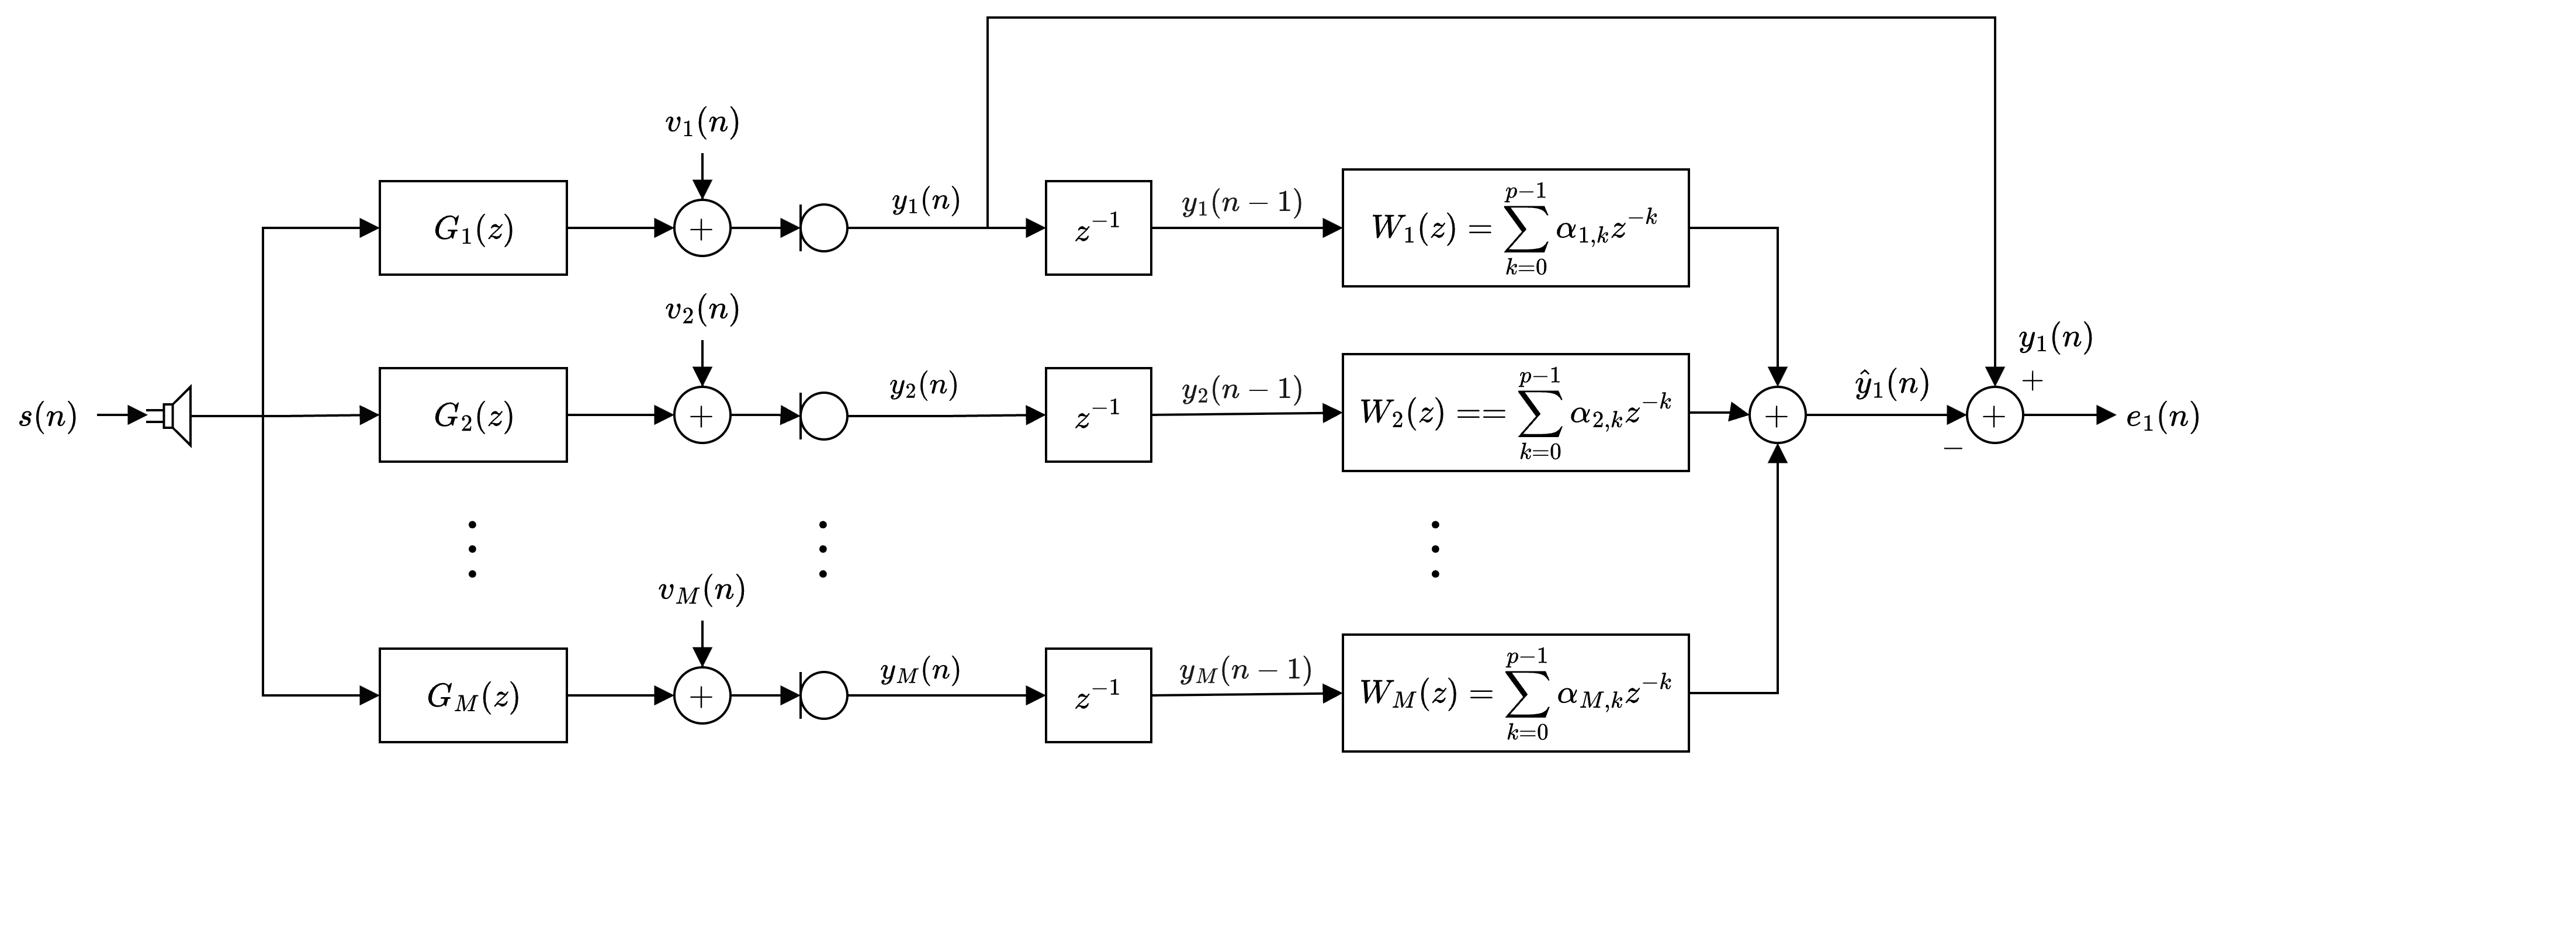
\includegraphics[width = \textwidth]{MC_LPC}
	\centering
	\caption{Block diagram for multichannel linear prediction applied to channel equalization, where an estimate of reverberant microphone signal 1 is produced by filtering and summing past samples of reverberant microphone signals 1-$M$}.
	\label{fig:MC_LPC}
\end{figure}

As shown, the current samples of $y_1(n)$ are estimated by filtering and summing the past $p$ samples of all $M$ microphone signals. Note that since all output signals reflect the same source data, $s(n)$, it is important that the output signals are time-aligned. This is necessary so that the window of source data included in the delayed signals, $\{y_1(n-1), \dots, y_M(n-1)\}$), indeed lags the data included in $y_1(n)$ by 1 sample. If the signals are not aligned in this way, the prediction error filter will cancel $y_1(n)$ instead of whitening it.

The prediction error signal $e_1(n)$ is thus

\noindent
\begin{equation}
	e_1(n) = y_1(n) - \hat{y}_1(n)) = y_1(n) -\sum_{m=1}^{M} \sum_{k=1}^{p} \alpha_{m,k} y_m(n-k) \label{eq:mc_lp_error}
\end{equation}

\noindent
which can be represented in vector form as

\begin{eqnarray}
	e_1(n)=y_1(n) - \sum_{k=1}^{p} \boldsymbol{\alpha}_k^T \boldsymbol{y}(n-k) \\
	e_1(n) = y_1(n) - \boldsymbol{\tilde{\alpha}}^T \boldsymbol{\tilde{y}}(n-1) \label{eq:mc_lp_error_vec}
\end{eqnarray}

\noindent
with
\begin{eqnarray}
	\boldsymbol{y}(n) = 
	\begin{bmatrix}
		y_1(n) &	y_2(n)  & \dots  & y_M(n)  \\
	\end{bmatrix}^T  \in  \mathbb{R} ^ {M \times 1} \\
	%
	\boldsymbol{\alpha}_k = 
	\begin{bmatrix}
		\alpha_{1,k} &	\alpha_{2,k} & \dots  & \alpha_{M,k} \\
	\end{bmatrix}^T  \in  \mathbb{R} ^ {M \times 1}
\end{eqnarray}

\noindent
and
\begin{eqnarray}
	\boldsymbol{\tilde{y}}(n-1) = 
	\begin{bmatrix}
		\boldsymbol{y}^T(n-1) &	\boldsymbol{y}^T(n-2)  & \dots  & \boldsymbol{y}^T(n-p)   \\
	\end{bmatrix}^T  \in  \mathbb{R} ^ {Mp \times 1}\\
	%
	\boldsymbol{\tilde{\alpha}} = 
	\begin{bmatrix}
		\boldsymbol{\alpha}^T_1 &	\boldsymbol{\alpha}^T_2  & \dots  & \boldsymbol{\alpha}^T_p \\
	\end{bmatrix}^T  \in  \mathbb{R} ^ {Mp \times 1}
\end{eqnarray}


It is more common, however, to formulate multichannel linear prediction as estimating the sample of a vector-valued signal, $\boldsymbol{y}(n)$, from it's past $p$ vector-valued samples. This results in a vector-valued error signal, $\boldsymbol{e}(n) = \begin{bmatrix} e_1(n) & e_2(n) & \dots& e_M(n) \end{bmatrix}^T$, defined as

\begin{eqnarray}
	\boldsymbol{e}(n) = \boldsymbol{y}(n) - \boldsymbol{\hat{y}}(n) = \boldsymbol{y}(n) - \sum_{k=1}^{p} \boldsymbol{A}_k \boldsymbol{y}(n-k)  \label{eq:mc_lp_error_parallel}
\end{eqnarray}

\noindent
where $\boldsymbol{A}_k \in  \mathbb{R} ^ {M\times M}$ prediction coefficient matrices for a $k$-sample delay. This can also be fully encapsulated in vector form as

\begin{equation}
	\boldsymbol{e}(n)= \boldsymbol{y}(n) - \boldsymbol{A}_{\mathrm{mc}} \tilde{\boldsymbol{y}}(n-1) \label{eq:mc_lp_error_vec_parallel}
\end{equation}

\noindent
where

\begin{eqnarray}
	\boldsymbol{A}_{\mathrm{mc}} = \begin{bmatrix}
		\boldsymbol{A}_1 & \boldsymbol{A}_2 & \dots& \boldsymbol{A}_p
	\end{bmatrix} \in \mathbb{R}^{M \times Mp}
\end{eqnarray}

\noindent
Note that the first row of Equation \ref{eq:mc_lp_error_vec_parallel} is exactly Equation \ref{eq:mc_lp_error_vec}. Similarly, row 2 represents the prediction of $y_2(n)$, row 3 represents the prediction of $y_3(n)$, and so on.

The multichannel versions of the prediction error filter, $\boldsymbol{A}_{\mathrm{pe,mc}}(z)$, and inverse filter, $\frac{1}{\boldsymbol{A}_{\mathrm{pe,mc}}(z)}$ are thus

\begin{eqnarray}
	\boldsymbol{A}_{\mathrm{pe,mc}}(z) = \boldsymbol{I} - \sum_{k=1}^{p} \boldsymbol{A}_k z^{-k} \label{eq:mc_pe_filter} \\
	%
	\frac{1}{\boldsymbol{A}_{\mathrm{pe,mc}}(z)} = \frac{1}{\boldsymbol{I} - \sum_{k=1}^{p} \boldsymbol{A}_k z^{-k}}
\end{eqnarray}

\noindent
where $\boldsymbol{I} \in \mathbb{R}^{M \times M}$ is the identity matrix. Note that these are vector-valued filters, i.e., 

\begin{equation}
	\boldsymbol{e}(z) = \boldsymbol{A}_{\mathrm{pe,mc}}(z) \boldsymbol{y}(z)
\end{equation}

\noindent
with 

\noindent
\begin{eqnarray}
	\boldsymbol{e}(z) = Z\{\boldsymbol{e}(n)\} = \begin{bmatrix} Z\{e_1(n)\} & \dots & Z\{e_M(n)\} \end{bmatrix}^T\\
	%
	\boldsymbol{y}(z) = Z\{\boldsymbol{y}(n)\} = \begin{bmatrix} Z\{y_1(n)\} & \dots & Z\{y_M(n)\} \end{bmatrix}^T
\end{eqnarray}

Like in Section \ref{lp_autocor}, we define a mean-squared error cost function, 

\begin{equation}
	J = E[\boldsymbol{e}^T(n)\boldsymbol{e}(n)]]
\end{equation}

\noindent
where the definition of the estimator for the expectation operator, $E[\cdot]$, distinguishes between the autocorrelation method and the covariance method. The optimal prediction coefficients are derived by minimizing $J$ (i.e., by setting $\partial J/\partial \alpha_{l,m,k}=0$, where $l$ is the channel being predicted, $m$ is the channel being used in prediction, and $k$ is the delay). 

Since each row of Eqauation \ref{eq:mc_lp_error_vec_parallel} represents the formulation of an independent Wiener Filter (Section \ref{wiener_filter}), assuming the microphone signals are stationary, the solution for each row of $\boldsymbol{A}_{\mathrm{mc}}$ (i.e., $\boldsymbol{\tilde{\alpha}}^T_m$) is given by

\begin{eqnarray}
	\boldsymbol{R}_{\boldsymbol{\tilde{y}}(n)\boldsymbol{\tilde{y}}(n)} \boldsymbol{\tilde{\alpha}}_m =
	\boldsymbol{r}_{\boldsymbol{\tilde{y}}(n-1)y_m(n)}  \\
	%
	(\boldsymbol{R}_{\boldsymbol{\tilde{y}}(n)\boldsymbol{\tilde{y}}(n)} \boldsymbol{\tilde{\alpha}}_m)^T =
	(\boldsymbol{r}_{\boldsymbol{\tilde{y}}(n-1)y_m(n)})^T \rightarrow
	%
	\boldsymbol{\tilde{\alpha}}^T_m  \boldsymbol{R}_{\boldsymbol{\tilde{y}}(n)\boldsymbol{\tilde{y}}(n)} =  \boldsymbol{r}^T_{\boldsymbol{\tilde{y}}(n-1)y_m(n)} %\\
	%\boldsymbol{\alpha}^T_m = \boldsymbol{r}^T_{\boldsymbol{\tilde{y}}(n-1)y_m(n)} R_{\boldsymbol{\tilde{y}}(n)\boldsymbol{\tilde{y}}(n)}^{-1}
\end{eqnarray}

\noindent
with

\begin{eqnarray}
	\boldsymbol{R}_{\boldsymbol{\tilde{y}}(n)\boldsymbol{\tilde{y}}(n)} = E[\boldsymbol{\tilde{y}}(n) \boldsymbol{\tilde{y}}^T(n] \in  \mathbb{R} ^ {Mp \times Mp}\\
	%
	\boldsymbol{r}_{\boldsymbol{\tilde{y}}(n-1)y_m(n)} = E[\boldsymbol{\tilde{y}}(n-1)y_m(n)] \in  \mathbb{R} ^ {Mp \times 1}
\end{eqnarray}

Packing all $M$ equations together we get the final solution for $A_{\mathrm{mc}}$,

\begin{eqnarray}
	\begin{bmatrix}
		\boldsymbol{\tilde{\alpha}}^T_1 \\
		\boldsymbol{\tilde{\alpha}}^T_2 \\
		\vdots \\
		\boldsymbol{\tilde{\alpha}}^T_M \\
	\end{bmatrix}
	\boldsymbol{R}_{\boldsymbol{\tilde{y}}(n)\boldsymbol{\tilde{y}}(n)} =
	\begin{bmatrix}
		\boldsymbol{r}^T_{\boldsymbol{\tilde{y}}(n-1)y_1(n)} \\
		\boldsymbol{r}^T_{\boldsymbol{\tilde{y}}(n-1)y_2(n)}\\
		\vdots \\
		\boldsymbol{r}^T_{\boldsymbol{\tilde{y}}(n-1)y_M(n)} \\
	\end{bmatrix} \\
	%
	\boldsymbol{A}_{\mathrm{mc}}\boldsymbol{R}_{\mathrm{mc}} = \boldsymbol{r}_{\mathrm{mc}} \label{eq:mc_yule_walker} \\
	%
	\boldsymbol{A}_{\mathrm{mc}} = \boldsymbol{r}_{\mathrm{mc}} \boldsymbol{R}_{\mathrm{mc}}^{-1}
\end{eqnarray}

\noindent
with

\begin{eqnarray}
	\boldsymbol{R}_{\mathrm{mc}} = E[\boldsymbol{\tilde{y}}(n) \boldsymbol{\tilde{y}}^T(n] = 
	\begin{bmatrix}
		\boldsymbol{R}_{\boldsymbol{yy}}(0)     & \boldsymbol{R}_{\boldsymbol{yy}}(1)    & \dots   & \boldsymbol{R}_{\boldsymbol{yy}}(p-1)  \\
		\boldsymbol{R}_{\boldsymbol{yy}}(1)      & \boldsymbol{R}_{\boldsymbol{yy}}(0)      & \dots   & \boldsymbol{R}_{\boldsymbol{yy}}(p-2) \\
		\vdots                               & \vdots                               & \ddots & \vdots \\
		\boldsymbol{R}_{\boldsymbol{yy}}(p-1) & \boldsymbol{R}_{\boldsymbol{yy}}(p-2)  & \dots   & \boldsymbol{R}_{\boldsymbol{yy}}(0) \\
	\end{bmatrix}  \in  \mathbb{R} ^ {Mp \times Mp} \\
	%
	\boldsymbol{r}_{\mathrm{mc}} = E[\boldsymbol{y}(n)\boldsymbol{\tilde{y}}^T(n-1)] = 
	\begin{bmatrix}
		\boldsymbol{R}_{\boldsymbol{yy}}(1)     & \boldsymbol{R}_{\boldsymbol{yy}}(2)     & \dots   & \boldsymbol{R}_{\boldsymbol{yy}}(p) 
	\end{bmatrix} \in  \mathbb{R} ^ {M \times Mp}
\end{eqnarray}

\noindent
where $\boldsymbol{R}_{\boldsymbol{yy}}(l)$ is the spatial correlation matrix of the microphone signals for lag $l$. I.e., 

\noindent
\begin{equation}
	\boldsymbol{R}_{\boldsymbol{yy}}(l) = E[\boldsymbol{y}(n) \boldsymbol{y}^T(n)] = 
	\begin{bmatrix} 
		r_{y_1y_1}(l)   & r_{y_1y_2}(l)  & \dots   & r_{y_1y_M}(l) \\
		r_{y_2y_1}(l)   & r_{y_2y_2}(l)& \dots    & r_{y_2y_M}(l)  \\
		\vdots     & \vdots      & \ddots  & \vdots  \\
		r_{y_My_1}(l)  & r_{y_My_2}(l) & \dots    & r_{y_My_M}(l) \\
	\end{bmatrix} \\
\end{equation}

\noindent
where $r_{y_i y_k}(l)=E[y_i(n) y_k(n-l)]$ is the cross-correlation between microphone signal $i$ and microphone signal $k$ at lag $l$. 

Equation \ref{eq:mc_yule_walker} is known as the multichannel Yule-Walker equation. Note that the multichannel spatio-temporal correlation matrix, $\boldsymbol{R}_{\mathrm{mc}}$, has a block-toeplitz form due to the assumption that the microphone signals are stationary. This shape is dependent on the selection of space-first packing in the multichannel spatio-temporal data vector, $\boldsymbol{\tilde{y}}(n)$, and enables usage of the block Levinson algorithm \citep[i.e., the multichannel Levinson algorithm, ][]{whittle1963fitting} which is a generalization of the traditional Levinson-Durbin algorithm to block-toeplitz systems of linear equations.

Similar to traditional single-channel linear prediction, the formulation of the multichannel Yule-Walker equation using estimates of autocorrelation (i.e., the autocorrelation method) has been shown to produce a stable linear prediction inverse filter, $\frac{1}{\boldsymbol{A}_{\mathrm{mc}}(z)}$ \citep{inouye1983modeling}. While this does not imply that the individual scalar prediction filters are minimum phase, it does imply that the autocorrelation method is a constrained solution. Therefore, like single-channel linear prediction, the covariance method may produce a more accurate model of the system, at the cost of increased computational complexity.

As previously mentioned, the multichannel prediction error filter (Equation \ref{eq:mc_pe_filter}) can be applied to the microphone signals to blindly equalize the RTF, but will also whiten the source. Moreover, if an equalizer is designed based on one source signal ($s_1(n)$), and then applied to a different one ($s_2(n)$), the autoregressive parameters of $s_1(n)$  will greatly distort (rather than whiten) $s_2(n)$, potentially increasing the perceived amount of reverberation. To compensate this undesired effect, a number of algorithms have been proposed which leverage spatial diversity to estimate the autoregressive properties of the source, separate from the channel.  Of particular note, there are two seminal appraoches: delay and predict (i.e., DAP) dereverberation \citep{triki2006delay} and linear-predictive multiple-input equalization (i.e., LIME) \citep{delcroix2007precise}.

DAP dereverberation is described in Figure \ref{fig:dap_block_diagram}. 

\begin{figure}[H]
	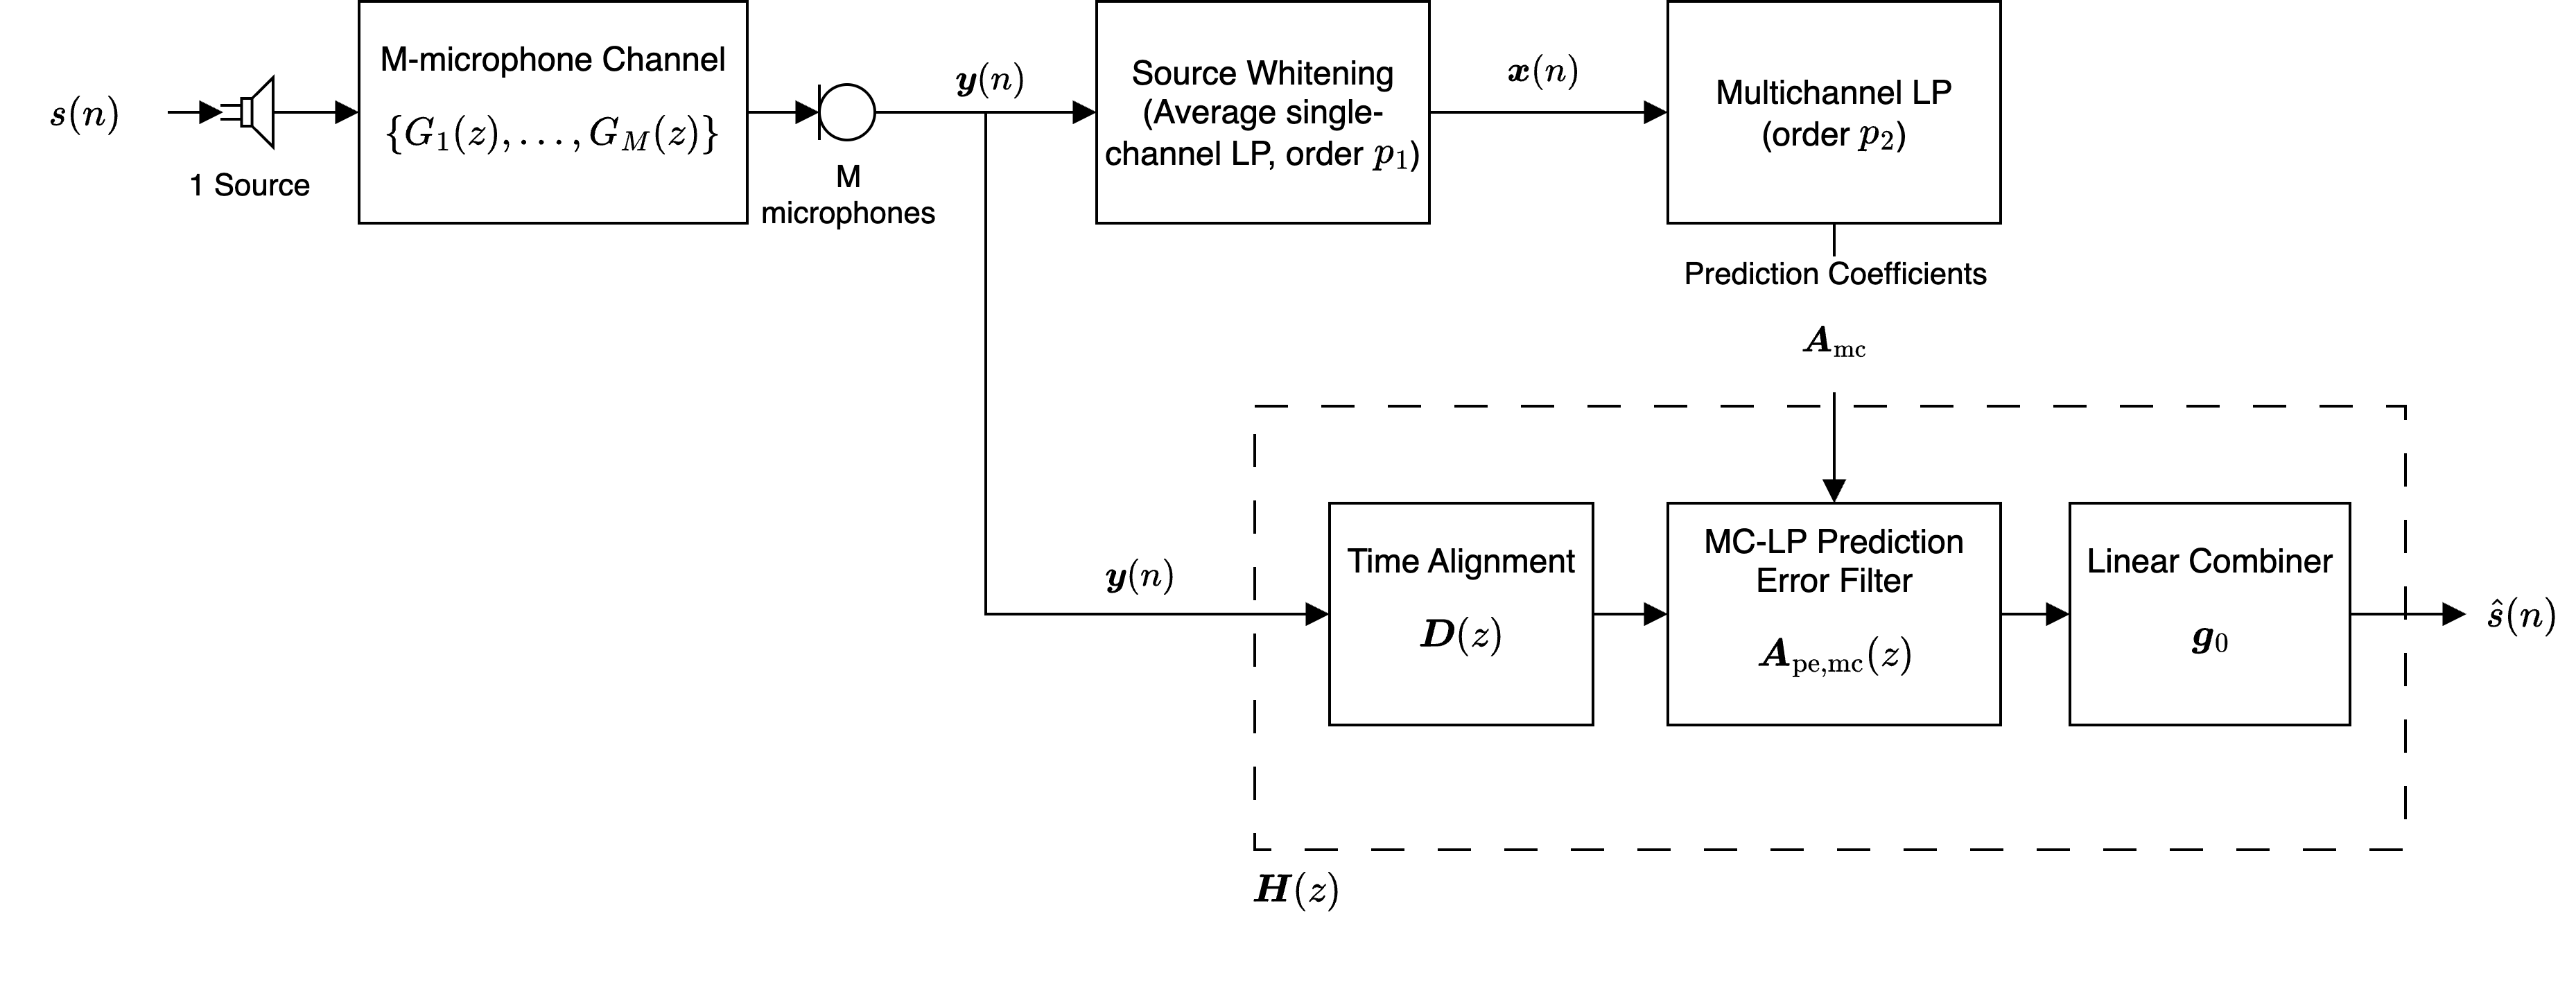
\includegraphics[width = 1.0\textwidth]{dap_block_diagram}
	\centering
	\caption{Block diagram for delay-and-predict derverberation \citep{triki2006delay}}
	\label{fig:dap_block_diagram}
\end{figure}


This approach consists of three stages:

\begin{enumerate}
	\item Source Whitening Stage: The AR parameters of the source are estimated and the corresponding prediction error filter is applied to each of the reverberant microphone signals, $\{y_1(n), \dots, y_M(n)\}$ (i.e., vector-valued $\boldsymbol{y}(n)$), thus whitening only the AR properties of the source. The result is a set of source-whitened reverberant microphone signals, $\{x_1(n), \dots, x_M(n)\}$ (i.e., vector-valued $\boldsymbol{x}(n)$).
	%
	\item Multichannel Linear Prediction Stage: The source-whitened reverberant microphone signals are used in Equation \ref{eq:mc_yule_walker} to compute the mutlichannel prediction coefficients, $\boldsymbol{A}_{\mathrm{mc}}$, and generate a multichannel prediction error filter, $\boldsymbol{A}_{\mathrm{pe,mc}}(z)$.
	%
	\item Dereverberation Stage: The multichannel prediction error filter is combined in series with a time-alignment filter and a linear combiner to form the full delay-and-predict equalizer, $\boldsymbol{H}(z)$, which is applied to the original reverberant microphone signals, $\boldsymbol{y}(n)$. Since this prediction error filter was computed using the source-whitened signals, it should not include the AR parameters of the source signal, and thus should not whiten the source part of the microphone signals. Therefore the resulting prediction error signal should only whiten the channel, thus fascilitating dereverberation.
\end{enumerate}

In the source whitening stage, the AR parameters of the source are estimated as those that minimize the single-channel prediction error for all $M$ microphone signlas. This is formulated as minimizing the sum of the single-channel prediction errors, i.e., the cost function is

\begin{equation}
	J = \sum_{m=1}^{M} E[ e_m^2(n) ] = \sum_{m=1}^{M} E[ y_m(n) - \sum_{k=1}^{p} \alpha_k y_m(n-k) ]
\end{equation}

Minimization of $J$ (i.e., setting $\frac{\partial J}{\partial \alpha_k} = 0$), assuming the microphone signals are stationary, the resulting normal equations are

\begin{eqnarray}
	\begin{bmatrix}
		\bar{r}_{yy}(0) & \bar{r}_{yy}(1) & \dots & \bar{r}_{yy}(p-1) \\
		\bar{r}_{yy}(1) & \bar{r}_{yy}(0) & \dots & \bar{r}_{yy}(p-2) \\
		\vdots               & \vdots              & \ddots & \vdots \\
		\bar{r}_{yy}(p-1) & \bar{r}_{yy}(p-2) & \dots & \bar{r}_{yy}(0)
	\end{bmatrix}
	\begin{bmatrix}
		\alpha_1 \\
		\alpha_2 \\
		\vdots \\
		\alpha_p
	\end{bmatrix} =
	\begin{bmatrix}
		\bar{r}_{yy}(1)  \\
		\bar{r}_{yy}(2)  \\
		\vdots \\
		\bar{r}_{yy}(p) 
	\end{bmatrix}
\end{eqnarray}

\noindent
where $\bar{r}_{yy}(l) = \sum_{m=1}^{M} r_{y_m y_m}(l) = \sum_{m=1}^{M} E[ y_m(n) y_m(n-l) ]$, i.e., the average autocorrelation accross all microphones.

In the dereverberation stage of the DAP algorithm, the actual multichannel equalizer filter, $\boldsymbol{H}(z)$, is computed as 

\begin{equation}
	\boldsymbol{H}(z) = \boldsymbol{g}_0 \boldsymbol{A}_{pe,mc}(z) \boldsymbol{D}(z)
\end{equation}

\noindent
where $\boldsymbol{A}_{pe,mc}(z)$ is the multichannel prediction error filter computed in the previous stage (Equation \ref{eq:mc_pe_filter}), $\boldsymbol{D}(z)$ is a diagonal matrix of delay elements ($\boldsymbol{D}(z) = \mathrm{diag} \{z^{-d_1} \dots z^{-d_M}\}$) used to time-align the microphone signals, and $\boldsymbol{g}_0$ is a weighting vector that computes a linear combination of the length-$M$ vector output of the multichannel prediction error filter. Together $D(z)$ and $\boldsymbol{g}_0$ effectively perform delay-weight-and-sum beamforming on equalized vector output of the multichannel prediction error filter. To generate $\boldsymbol{D}(z)$, the time delay between the microphones must be estimated, which is a well understood topic with many practical approaches. In the original DAP algorithm, the linear combiner weights $\boldsymbol{g}_0$ (as denoted by the variable symbol) were selected to be the vector coefficient of the SIMO channel, i.e., $\boldsymbol{g}_0 = \begin{bmatrix} g_1(0) \dots g_M(0) \end{bmatrix} ^T$. It was shown that $\boldsymbol{g}_0$ can be blindly estimated with reasonable accuracy as the eigenvector corresponding to the largest eigenvalue of the autocorrelation matrix corresponding to the multichannel prediction error signal from the second algorithm stage. I.e., $\boldsymbol{g}_0$ is estimated as the principal component of the matrix $\boldsymbol{R}_{\tilde{\boldsymbol{x}} \tilde{\boldsymbol{x}}} = E[ \tilde{\boldsymbol{x}}(n) \tilde{\boldsymbol{x}}^T(n) ]$, where

\begin{equation}
	\tilde{\boldsymbol{x}}(n) = \boldsymbol{x}(n) - \hat{\boldsymbol{x}}(n) = \boldsymbol{x}(n) - \sum_{k=1}^{p} A_k \boldsymbol{x}(n-k)
\end{equation}

The final output of the DAP equalizer is thus computed as 

\begin{equation}
	\hat{S}(z) = \boldsymbol{H}(z) \boldsymbol{y}(z) 
\end{equation}

\noindent
or equivalently

\begin{equation}
	\hat{s}(n) = \sum_{m=1}^{M} g_m(0) s_m(n-d_m) \\
\end{equation}

\noindent 
with

\begin{equation}
	\begin{bmatrix} \hat{s}_1(n-d_1) \\ \dots \\ \hat{s}_M(n-d_M) \end{bmatrix} =
	\boldsymbol{y}(n) - \sum_{k=1}^{p} A_k \boldsymbol{y}(n-k)
\end{equation}

\cite{triki2006delay} explained that the prediction order for the multichannel linear prediction stage ($p_2$) should be selected such that it meets the MINT requirements, i.e., $p_2=L_g/(M-1)$, where $L_g$ is the length of the FIR channels. It was suggested that the prediction order for the source-whitening stage ($p_1$) should be selected such that that the source is sufficiently undistorted by the multichannel prediction error filter. For a sample rate of \qty{8}{\kilo\hertz}, $p_1=100$ was considered sufficient. However, it should be noted that the higher order AR parameters of the source (i.e., higher than those reflected by $p_1$) will still be included in the multichannel prediction error filter, distorting the estimate of the true system inverse, which will limit its applicability to other source signals. Additionally, note that the source signal does not need to be stationary, but rather it is only important that the same window of speech is used in the estimation of the source AR parameters and the multichannel prediction coefficients. As such, it was recommended that the entire speech stimulus be used in analysis so as to reduce estimation variance.


In the LIME algorithm, the multichannel prediction coefficients are estimated directly from the reverberant microphone signals, $\{y_1(n), \dots, y_M(n)\}$. The multichannel prediction error filter thus whitens the source signal, and then an un-whitening filter is applied after. \cite{delcroix2007precise}, showed that under a certain matrix formulation, the multichannel prediction coefficients corresponding to the reverberant microphone signals and the source AR parameters can be independently extracted.

As per the MINT, both DAP and LIME require that the RTFs have no common zeros, and additionally require that the AR parameters of the channels (i.e., the effective poles) do not overlap. If the effective poloes of the RTFs overlap, these will be wrongly associated with the source and will not be equalized. As channel order increases (i.e., longer reverberation times), the concentration of zeros around the unit circle increases and the likelihood of overlapping or numerically overlapping zeros increases, thus requiring more microphones to acheive reasonable performance. When formulated as MIMO prediction of signal vector $\boldsymbol{y}(n)$ (i.e., as in Equation \ref{eq:mc_lp_error_parallel}), there is potential to constrain the solution so that the phase of the individual dereverberated signals in $\boldsymbol{e}(n)$ are not distorted. In this way the output of the algorithm can be input to further spatial processing and/or spatial cues can be preserved to aid in speech perception (Section \ref{perceptual_adaptations}) 

Several extensions of DAP and LIME have been proposed, such as methods for compensating the effects of additive noise \citep[e.g., ][]{triki2007multivariate}, alternative methods for combining the $M$ dereverberated signals in $\boldsymbol{e}(n)$ \citep[e.g., ][]{triki2008robust}, and adaptive extensions which generally use RLS for adaptation and often operate in the FFT/subband domain \citep[e.g., ][]{jukic2016adaptive, jukic2016general}. Usage of delayed linear prediction \citep[i.e., multi-step linear prediction originally presented by ][]{gesbert1997robust} has also been proposed, whereby a multi-sample delay is applied to the signals being used in prediction instead of the traditional single-sample delay. Delayed linear prediction allows algorithms to avoid cancelling the early reflections and also reduces the over-whitening effects of linear prediction, but is more computationally complex. 

Multichannel linear predictive techniques are often considered to be the most practical approach to reverberation cancellation due to the fact they can be performed in a truly blind manner, not requiring any knowledge of the source or channel order, and since linear prediction is a well understood topic that is easily extensible to an adaptive framework. These approaches have generally proven to perform well for shorter reverberation times, but their performance diminishes with increased reverberation due to estimation variance and the massive amounts of data needed to reduce estimation variance. Additionally, the underlying assumption that RTFs are time-invariant severly limits performance in practice since real acoustics are highly time varying. For longer reverberation times, where channel orders can reach up to tens of thousands (E.g., a T60 of \qty{2}{\second} at a sample rate of \qty{16}{\kilo\hertz} represents an RIR of length \qty{32}{\kilo samples}), solving the normal equations also becomes impractical due to the massive matrices involved. However, this challenge can be reduced at the cost of decreased performance by using stochastic gradient descent algorithms which do not require matrix inversion.

To manage the performance limitations of these approaches, several authors have suggested the enhancement of multichannel linear predictive inverse filtering with a spectral subtraction post-processing stage to reduce residual late reflections \citep[e.g., ][]{furuya2007robust}. Some authors have also suggested using linear prediction to estimate reverberation, but then removing it via spectral subtraction rather than inverse filtering \citep[e.g., ][]{kinoshita2007multi, nakatani2008blind, nakatani2010speech}, claiming that this approach is more robust to imperfections in system estimate. 


\subsubsection{Blind System Identification Using Estimation Theory}

In recent years, significant research has gone into blind reverberation cancellation techniques that use statistical estimation methods for BSI. One of the most seminal appraoches is the so-called weighted prediction error algorithm \citep[i.e., WPE ][]{nakatani2008blind, nakatani2010speech}, which is one of the most common algorithms applied in practice. In this multichannel method, the reverberant speech signal is conceptually divided into a "desired" direct/early component and a late reverberant component, and an estimate of the late reverberant component is subtracted from the observed signal. A single reverberant microphone signal is modeled as a multichannel delayed linear-predictive process as a function of all microphone signals, with a prediction delay matching the defined boundary between early and late reflections. The desired component is modeled as a Gaussian process that is short-time quasi-stationary with time varying variance over longer time. The delayed prediction coefficients of the process are estimated via maximum likelihood estimation, and the resulting prediction error filter is used to subtract the late reflections. The technique was also extended to the STFT/subband domains to reduce computational complexity.

A number of appraoches have also been proposed which setup Bayesian prioirs \citep[e.g., ][]{hopgood2005models}, with some priors more recently being based on the assumed sparsity of the time-frequency representation of clean speech \citep{jukic2015multi, jukic2016general}.

Several authors have also enhanced this concept with techniques for modeling the time-varying nature of the acoustics. This has been done by treating the prediction coefficients (i.e., the model parameters) themselves as random variables with parameters to be estimated. Parameter estimation in this case has been proposed primarily using recursive estimation procedures such as Kalman filtering \citep[e.g., ][]{braun2016online, schmid2014variational}. The simplest example of such a model is the so-called random-walk time-varying all-pole system, where individual poles are modeled as having Gaussian variation about their true value/mean. The ability of a probablistic framework to include modeling of the time-varying nature of acoustic represents a major potential benefit of these appraoches. Similarly, the clean speech source signal can be assigned a source-filter model, and the time-varying vocal tract can be modeled probablistically \citep{grenier2003time}. In this way the time-varying nature of speech can be leveraged rather than simply modeling the long-term statistics of speech as is done in non-probablistic approaches. Since as noise model can also be included in the setup, probablistic approaches tend to be less sensitive to noise.
 
Probablistic methods for estimating the clean speech and/or channel generally tend to outperform traditional inverse filtering appraoches such as delay-and-predict/LIME dereverberation, especially in non-stationary reverberant environments and in higher levels of reveberation or noise. However, these approaches are also incredibly complex computationally, often making them less practically applicable.

\section{Summary and Thesis Goals}

The previous two chapters outlined the perceptual motivation for dereverberation, and existing dereverberation algorithms. It was discussed that beamforming and statistical speech enhancement methods for reverberation suppression have proven to be computationally efficient and practical approaches to reducing the perceptual impacts of reverberation. However, due to their simplicity and limitations in their formulation, their performance is somewhat limited. On the other hand, multichannel reverberation cancellation methods have potential to perfectly remove reverberation as dictated by the MINT, but their performance at long reverberation times is limited, especially in non-stationary/noisy environments due to the underlying blind system identification problem. It was discussed that multichannel linear prediction methods to blind system identification show the most promise, but still face the same limited performance issues, and solving the underlying linear prediction normal equations represents a massive computational cost. As such, many practical/effective approaches to dereverberation use multichannel linear predictive blind deconvolution to cancel the strong early part of the RIR, and are enhanced with statistical speech enhancement post-processing to suppress the diffuse/weak late tail of the RIR.

The goal set for this thesis was to provide a physiologically motivated perceptual analysis of the performance of multichannel linear prediction approaches to reverberation cancellation under practical conditions. For a case study, the delay-and-predict algorithm proposed by \cite{triki2006delay} was implemented and parameter-tuned for efficacy (Chapter 3), and its performance was assessed (Chapter 4). 